
\let\accentvec\vec
\documentclass[]{llncs}
\usepackage{colortbl}
\usepackage{silence}
\WarningFilter{todonotes}{The length}
\WarningFilter{caption}{Unsupported}
\WarningFilter{caption}{Forced redefinition}
\WarningFilter{caption}{The option}
\WarningFilter{caption}{Unknown document}

\let\spvec\vec
\let\vec\accentvec
\usepackage{amsmath}
\let\vec\spvec

\usepackage{url}
\usepackage{hyperref}
\usepackage{array}

\usepackage{caption}
%\usepackage[position=t]{subcaption}
\captionsetup{compatibility=false}
\usepackage{subcaption}
%\usepackage[caption=false]{subfig}

\usepackage{array}
\usepackage{cite}
\usepackage{amsmath,amssymb,amsfonts}
\usepackage{algorithmic}
\usepackage{graphicx}
\newsavebox{\imagebox}
\usepackage{textcomp}
\usepackage{xcolor}
\usepackage{listings}
\usepackage{lstautogobble}
\usepackage[listings,skins,breakable,raster,most]{tcolorbox}
\usepackage{numprint}
\usepackage{tikz}
\usetikzlibrary{positioning,shapes,arrows,fit,backgrounds}
\usepackage{booktabs}
\usepackage{multirow}
\usepackage{soul}
\usepackage{tabularx}
\usepackage{mathtools}

\usepackage{cleveref}
\crefname{codecount}{Code}{Codes}

\usepackage{todonotes}
\newcommand{\jk}[1]{\todo[inline]{JK:\@#1}}
\newcommand{\eb}[1]{\todo[inline]{EB:\@#1}}

\definecolor{tabhcolor}{rgb}{0.63, 0.79, 0.95}
\newcolumntype{$}{>{\global\let\currentrowstyle\relax}}
\newcolumntype{^}{>{\currentrowstyle}}
\newcommand{\rowstyle}[1]{\gdef\currentrowstyle{#1}%
	  #1\ignorespaces
	}




\usepackage{graphicx}
\graphicspath{%
	{./pictures/}
}

\lstset{%
	numberbychapter=false,
	belowskip=-10pt,
	aboveskip=10pt,
}

\lstdefinestyle{lstcodebox}{%
	basicstyle=\scriptsize\ttfamily,
	autogobble=true,
	tabsize=2,
	captionpos=b,
	float,
}

\renewcommand{\ttdefault}{pcr}
\lstdefinestyle{instylebf}{%
	basicstyle=\bfseries\scriptsize\ttfamily,
}

\lstdefinestyle{instyle}{%
	basicstyle=\scriptsize\ttfamily,
}

\lstdefinestyle{lstcommon}{ %
%\lstdefinestyle{sig}{ %
  %backgroundcolor=\color{white},   % choose the background color; you must add \usepackage{color} or \usepackage{xcolor}; should come as last argument
  basicstyle=\fontsize{8}{8}\ttfamily,        % the size of the fonts that are used for the code
  breakatwhitespace=false,         % sets if automatic breaks should only happen at whitespace
  breaklines=true,                 % sets automatic line breaking
  captionpos=n,                    % sets the caption-position to bottom
  %commentstyle=\color{mygreen},    % comment style
  deletekeywords={...},            % if you want to delete keywords from the given language
  %escapeinside={\%*}{*)},          % if you want to add LaTeX within your code
  extendedchars=true,              % lets you use non-ASCII characters; for 8-bits encodings only, does not work with UTF-8
  frame=none,                    % adds a frame around the code
  keepspaces=true,                 % keeps spaces in text, useful for keeping indentation of code (possibly needs columns=flexible)
  keywordstyle=\bf\ttfamily,       % keyword style
  language=C,                 % the language of the code
  morekeywords={*,...},           % if you want to add more keywords to the set
  %numbers=left,                    % where to put the line-numbers; possible values are (none, left, right)
  numbersep=5pt,                   % how far the line-numbers are from the code
  %numberstyle=\tiny\color{mygray}, % the style that is used for the line-numbers
  rulecolor=\color{black},         % if not set, the frame-color may be changed on line-breaks within not-black text (e.g. comments (green here))
  showspaces=false,                % show spaces everywhere adding particular underscores; it overrides 'showstringspaces'
  showstringspaces=false,          % underline spaces within strings only
  showtabs=false,                  % show tabs within strings adding particular underscores
  stepnumber=1,                    % the step between two line-numbers. If it's 1, each line will be numbered
  %stringstyle=\color{mymauve},     % string literal style
  tabsize=2,                    % sets default tabsize to 2 spaces
  title=\lstname                   % show the filename of files included with \lstinputlisting; also try caption instead of title
}


\lstset{ %
  autogobble=true,
  backgroundcolor=\color{white},   % choose the background color; you must add \usepackage{color} or \usepackage{xcolor}
  basicstyle=\scriptsize\ttfamily,       % the size of the fonts that are used for the code
  breakatwhitespace=false,         % sets if automatic breaks should only happen at whitespace
  breaklines=true,                 % sets automatic line breaking
  captionpos=b,                    % sets the caption-position to bottom
  %commentstyle=\color{green},    % comment style
  deletekeywords={...},            % if you want to delete keywords from the given language
  escapeinside={(*}{*)},          % if you want to add LaTeX within your code
  extendedchars=true,              % lets you use non-ASCII characters; for 8-bits encodings only, does not work with UTF-8
  frame=none,                    % (none, single) adds a frame around the code
  keepspaces=true,                 % keeps spaces in text, useful for keeping indentation of code (possibly needs columns=flexible)
  keywordstyle=\color{blue},       % keyword style
  language=Octave,                 % the language of the code
  otherkeywords={*,...},           % if you want to add more keywords to the set
  %numbers=left,                    % where to put the line-numbers; possible values are (none, left, right)
  numbersep=5pt,                   % how far the line-numbers are from the code
  numberstyle=\tiny\color{gray}, % the style that is used for the line-numbers
  rulecolor=\color{black},         % if not set, the frame-color may be changed on line-breaks within not-black text (e.g. comments (green here))
  showspaces=false,                % show spaces everywhere adding particular underscores; it overrides 'showstringspaces'
  showstringspaces=false,          % underline spaces within strings only
  showtabs=false,                  % show tabs within strings adding particular underscores
  stepnumber=1,                    % the step between two line-numbers. If it's 1, each line will be numbered
  stringstyle=\color{blue},     % string literal style
  tabsize=2,                     % sets default tabsize to 2 spaces
  title=\lstname,                  % show the filename of files included with \lstinputlisting; also try caption instead of title
}


\begin{document}

\title{Classifying Temporal Characteristics of Job I/O Patterns Using Machine Learning Techniques}


\institute{%
DKRZ -- \email{betke@dkrz.de}%
\and University of Reading--%
\email{j.m.kunkel@reading.ac.uk}%
}

\author{Eugen Betke \inst{1} \and  Julian Kunkel\inst{2}}

\maketitle

\begin{abstract}
Every day, supercomputers execute 1000s of jobs with different characteristics.
Data centers monitor the behavior of jobs to support the users and improve the infrastructure, for instance, by optimizing jobs or by determining guidelines for the next procurement.
The classification of jobs into groups that express similar run-time behavior aids this analysis as it reduces the number of representative jobs to look into.
This work utilizes machine learning techniques to cluster and classify parallel jobs based on the similarity in their temporal I/O behavior.
Our contribution is the qualitative and quantitative evaluation of different I/O characterizations and similarity measurements and the development of a suitable clustering algorithm.

In the evaluation, we explore I/O characteristics from monitoring data of one million parallel jobs and cluster them into groups of similar jobs.
Therefore, the time series of various IO statistics is converted into features using different similarity metrics that customize the classification.

When using general-purpose clustering techniques, suboptimal results are obtained.
Additionally, we extract phases of IO activity from jobs.
Finally, we simplify the grouping algorithm in favor of performance.
We discuss the impact of these changes on the clustering quality.
\end{abstract}

\textbf{Keywords: }IO fingerprinting, performance analysis, monitoring

\section{Introduction}
Scientific large-scale applications of different domains have different needs for I/O and, thus, exhibit a variety of access patterns on storage.
Even re-running the same simulation may lead to different behavior.
We can distinguish between a temporal behavior, i.e., the operations performed over time such as long read/write phases, bursty I/O pattern, and concurrent metadata operations, and spatial access pattern of individual processes of the application as they can be, e.g., sequential or random.

On different supercomputers, the same I/O patterns may result in different application runtimes depending on the nature of the access pattern.

For example, machines equipped with burst buffers \cite{10.1007/978-3-030-02465-9_9, 7004215} may significantly reduce application runtimes by absorbing bursty I/O traffic.
I/O congestion and file system performance degradation can occur when several I/O intensive jobs are running on the same machine at the same time.
I/O aware schedulers, like CARS~\cite{LIANG201925} and Flux~\cite{flux}, implement new scheduling strategies that utilize I/O metrics.
The analysis of I/O is important not only when I/O begins to take a considerable amount of application runtime but when I/O patterns begin to degrade the performance of the shared file system affecting runtimes of other applications and worsening user experience by unresponsive file systems~\cite{10.1007/978-3-030-02465-9_5}.

Understanding the exhibited I/O behavior and implications on the system would give users and administrators information to support analysis by revealing deficiencies and may indicate the potential for I/O optimization.
Knowing the potential for optimization is important for the support staff, as it allows them to identify applications that benefit from I/O optimizations.
For example, a widely used parallel application that still utilizes sequential I/O might be cost-efficient to optimize.

The main question is how to identify such applications automatically from the observed data.
Non-intrusive capturing of I/O metrics and the analysis can be challenging in many aspects.
Firstly, in order to find optimization potential, data must be recorded in an appropriate level of detail to retain temporal characteristics.
While capturing statistics on node level is supported by many monitoring tools, e.g., LASSi~\cite{sivalingam2019lassi}, Darshan\cite{hpcdarshan}, and SIOX\cite{TSACAMAOOP14}.
Detailed metrics on file level are more difficult to obtain.
A widespread method is re-implementation and pre-loading of an I/O interface, which contains monitoring code.

However, recording the data isn't enough, the obtained data must be processed but the manual analysis is infeasible as the number of jobs is large -- Monitoring systems of HPC systems record data of ten thousand jobs each day.
Hence a semi-automatic approach is required to reduce the number of jobs to investigate.

In a previous paper, we proposed a semi-automatic way to find relevant jobs by computing relevant job characteristics from time series of job behavior.
Basically, support staff could then focus on those IO-intense jobs that express certain metrics the most.
Here, we extend the approach by grouping similar jobs based on profiles and IO-phases in order to simplify the investigation effort.

In different disciplines, machine learning methods have proven to be powerful tools to extract new information from large data sets.
Therefore, we explore clustering strategies on monitoring data, to reveal hidden information.

This paper is organized as follows: Section 2 outlines the preliminary work and provides background knowledge that is important to understand the next sections.
In Section 3, we discuss the key problem we are dealing with.
In Section 4, we introduce\ alternative approaches for the clustering, as different goals for the analysis require different distance metrics, we discuss the variety of approaches.
We start with a simple solution and increase complexity.
The results and discussion are attached to the methodology of each solution as subsections.
Finally, in Section 5 we summarize the results.


\section{Preliminary Work}
The German Climate Computing Center (DKRZ) maintains a monitoring system that gathers various statistics from the Mistral HPC system.
Mistral has 3,340 compute nodes, 24 login nodes, and two Lustre file systems (lustre01 and lustre02) that provide a capacity of 52 Petabyte.
The monitoring system is made up of open source components such as Grafana, OpenTSDB, and Elasticsearch but also includes a lightweight self-developed data collector that captures continuously node statistics - we decided to implement an own collector when analyzing the overhead of existing approaches.
Additionally, the monitoring system obtains various job meta-information from the Slurm workload manager and injects selected log files.

Our motivation for automatic analysis of parallel jobs is the monitoring situation at DKRZ.
Mistral runs around 10.000 jobs a day, which is too much for manual analysis.
In the previous work~\cite{iocats2020}, we found a way to identify I/O intensive jobs and jobs with inefficient usage by deriving statistics from the node-level statistics.
This information can aid the procurement of new HPC systems or support the extension of an existing one.
While this approach helps to find individual jobs, it doesn't provide a global overview, which might be more important for making decisions at the data center perspective.
For example, a discovery of a large group of I/O-intensive and bursty applications would suggest attaching a burst buffer to the storage, to improve application runtimes.
In this paper, we take up the idea of I/O categorization from the previous work, where we partition job runtime into equal size segments and map them into three categories (LowIO, HighIO, and CriticalIO), and continue our work to obtain a global overview.

A difference to previously utilized job statistics is that this time Lustre proc files on Mistral doesn't offer Object Storage Client (osc) counters, since a major upgrade of Lustre file system from version 2.7 to 2.11.
Thus, instead of 13 metrics, this time our data contains only 9 metrics.

Understanding of the following work requires an understanding of data format, that is formed by segmentation and categorization of raw monitoring data.
Segmentation is a pre-processing step that splits data into equal-sized segments and computes a mean performance for each segment.
This stage preserves the performance units (e.g., Op/s, MiB/s) for each metric.
As further calculations that involve different metrics is difficult for different metrics,, we introduced a categorization\textbf{ pre-processing} step that takes into account the performance of the underlying HPC system and assigns an ordered category to each segment.
It takes the mean performance, that was calculated in the previous step, and assigns one of the three categories (LowIO = 0, HighIO = 1 and CriticalIO = 4).
The category split points are based on the histogram of the obtained values~\cite{iocats2020}.
This node-level data can then used to compute job-statistics by aggregating across time or nodes.

In summary, this data representation has the following key advantages for data analysis.
The ordered categories make the calculations between different metrics feasible, which is not possible with raw data.
Furthermore, the domains are equally scaled and compatible, because the values are between 0 and 4, and a value has a meaning.
Besides, the resulting data representation is much smaller compared to the raw data.
This allows us to apply compute-intensive algorithms to large datasets.
Finally, irrelevant data is hidden by the LowIO category and doesn't distract from significant parts of jobs.

In our previous work, we computed three high-level metrics per job that aid users to understand job profiles: 

\begin{itemize}
	\item \textbf{Job-I/O-Balance:} indicates how I/O load is distributed between nodes during job runtime.
	\item \textbf{Job-I/O-Utilization:} shows the average I/O load during I/O-phases.
	\item \textbf{Job-I/O-Problem-Time} is the fraction of job runtime that is I/O-intensive; it is approximated by the fractions of segments that are considered I/O intensive.
\end{itemize}

\begin{figure}
	\centering
	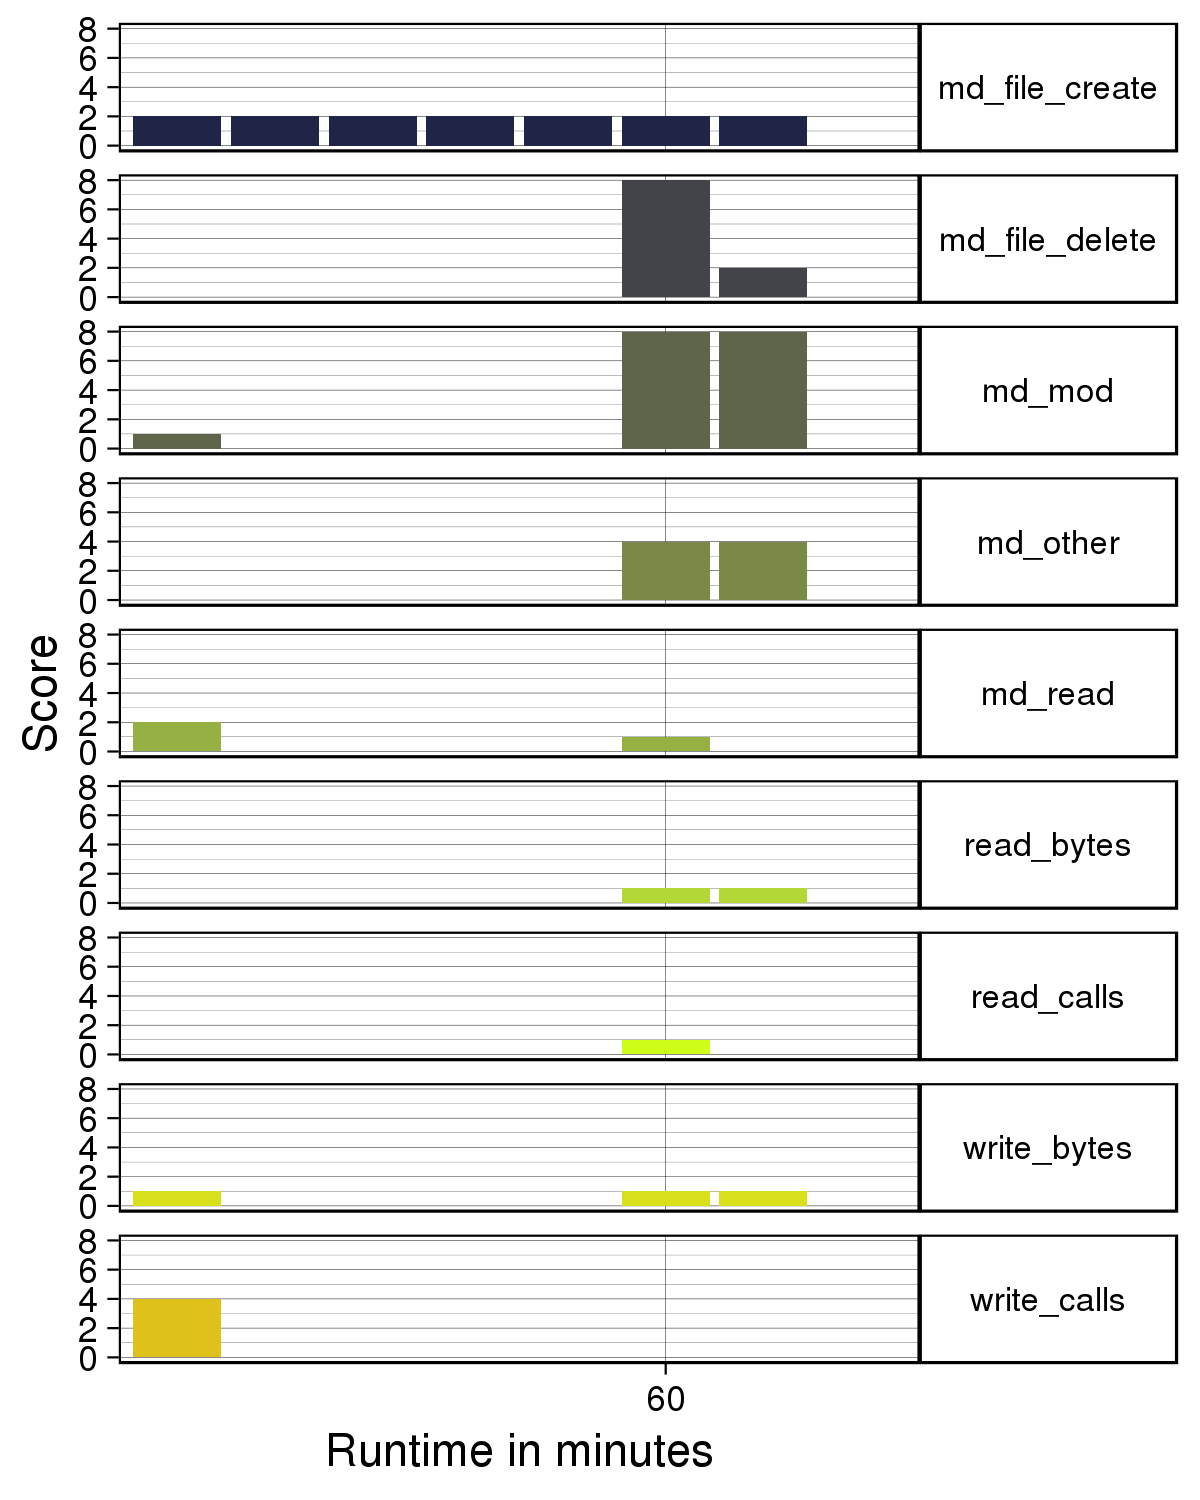
\includegraphics[width=2.02in,height=2.52in]{./media/image4.png}
	\caption{Metric Level View of an Example Job. Score is the sum of individual node scores.}
	\label{fig:seg_example}
\end{figure}

In \Cref{fig:seg_example}, we can see the temporal behavior for this particular job when summing up the node-level metrics.
We call \textbf{an I/O phase a contiguous sequence of non-zero segments} (where the score of the segment is larger than zero).
For example, in the figure, we can see one phase for md\_file\_create, and two phases for md\_mod (one short and non-intrusive at the beginning, and one critical around 60 minutes).

When looking at categorization at the metric level, i.e., after reduction of the nodes and file system dimensions, we can observe that many jobs exhibit I/O phases. 

\section{Similarity Between Jobs}
The raw monitoring data of a job in our environment at DKRZ, we obtain a time series of 9 metrics per node, each metrics sampled at five seconds intervals.
When comparing the time series of such metrics between two jobs, the key question is how do we define the similarity between multiple time series.
By applying dimensionality reduction techniques such as PCR, we can reduce the complexity and potentially obtain a similar representation for, e.g., two time series, but cannot make relevant distinctions between them.

First, we need to discuss the similarity of IO patterns from the user perspective.
In \Cref{fig:typ_io:1}, \Cref{fig:typ_io:2}, and \Cref{fig:typ_io:3} we illustrate the time series of two metrics for three different jobs.
The figures show the typical behavior of parallel applications, computation is interrupted by regular I/O phases - by phase, we mean a consecutive segment of time in which  certain behavior is exhibited, i.e., the statistics are similarly.

Actually,\ the shape of I/O phases depends on data view.
By applying dimension reduction techniques, I/O phases from different dimensions can be joined together.
Although several different aggregations are possible, in this work we focus on  I/O phases on metrics, i.e, we aggregate nodes and file system dimensions.
Identification of I/O phases shows that a substantial number of jobs has several of them.

From the user support side, we might be interested in grouping similar suboptimal jobs and aim to provide one recipe to optimize all that exhibit such a behavior.
Similarly, we might be interested to optimize the pattern for a single I/O phase.
We may be interested to ignore computation time and focus on I/O phases only.
Regardless of the segment of the time series we look at, we naively would consider an IO pattern to be identical if the time series for all metrics of one job is identical to those of another job.
Unfortunately, the obtained measurements vary due to the nature of parallel applications and the environment of the data center they are executed.
In practice, different jobs show a different runtime, and even when re-running the same job, the obtained time series varies.

\begin{figure}
	\centering
	 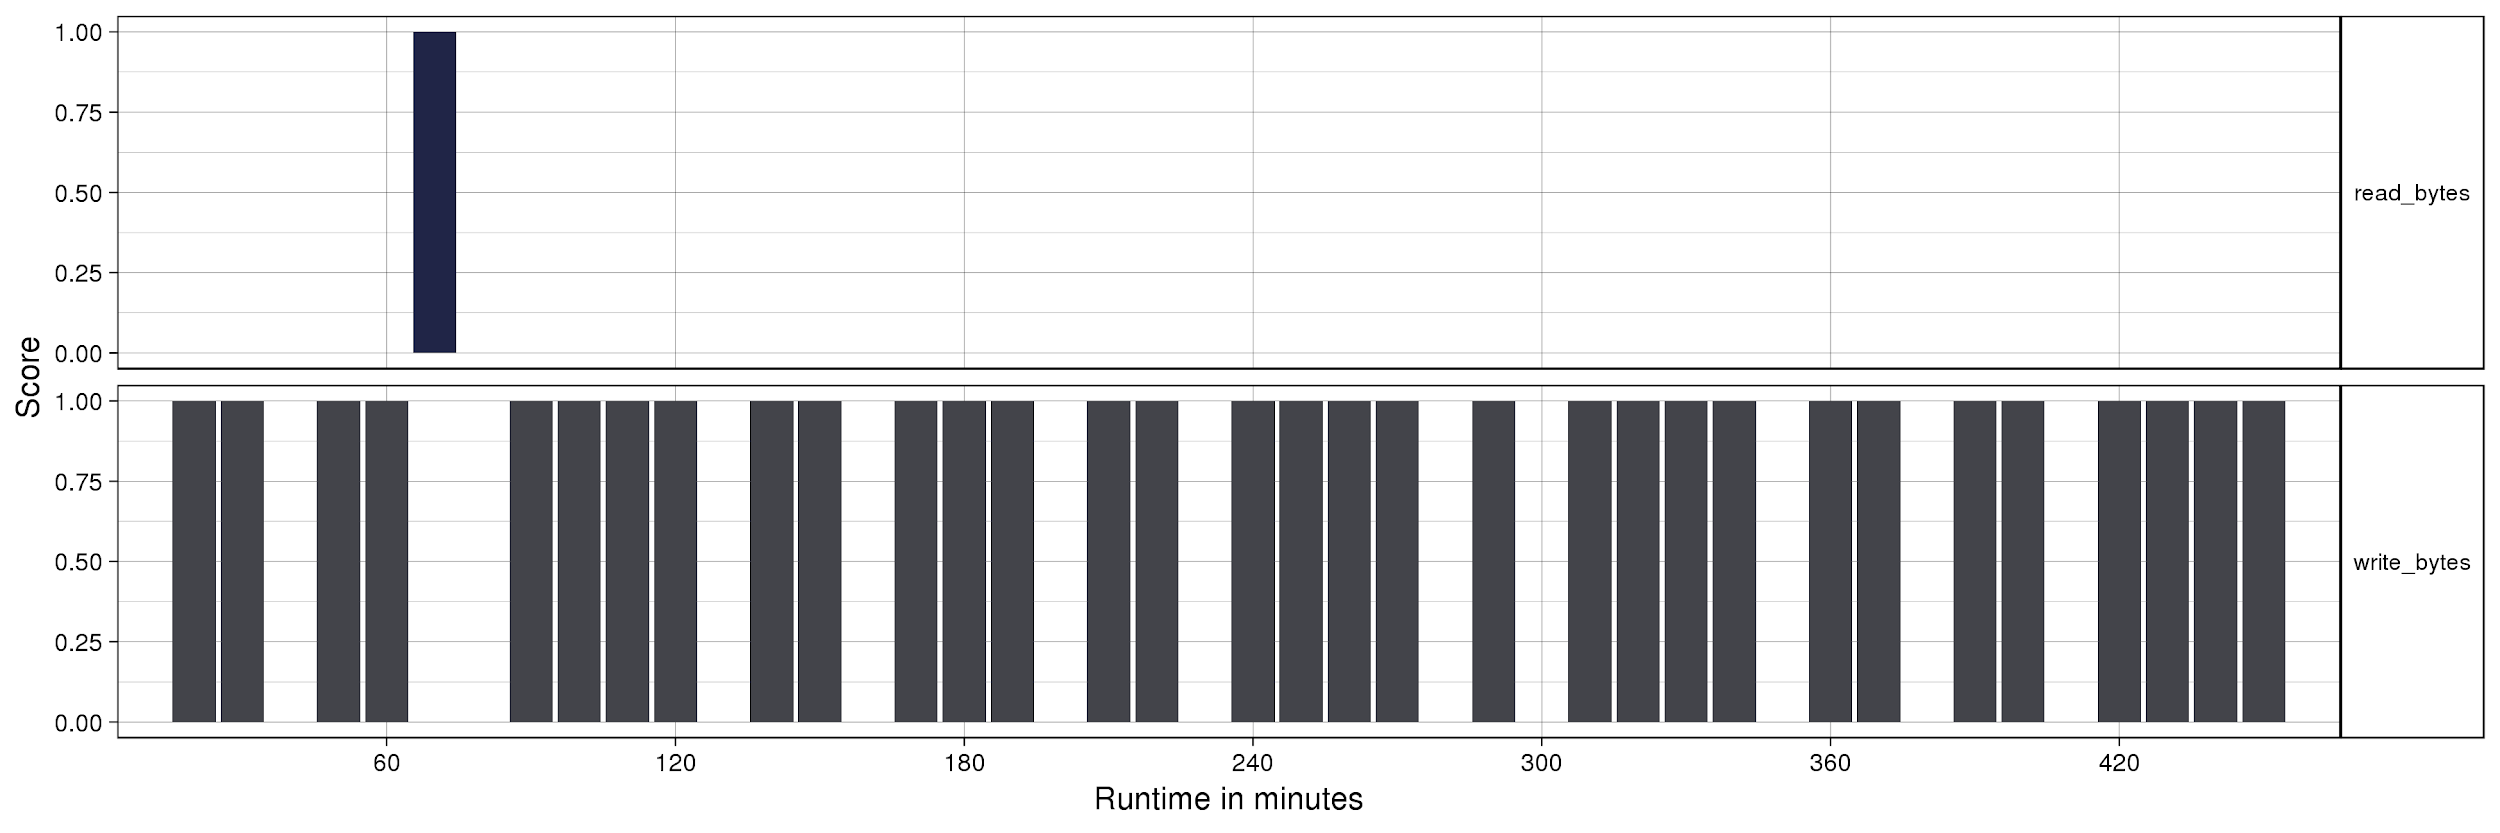
\includegraphics[width=4.61in,height=1.54in]{./media/image27.png}
	 \caption{Figure 2. Monitoring data of a 13 node job. Score is the sum of individual node scores.}
	 \label{fig:typ_io:1}
\end{figure}

\begin{figure}
	\centering
	 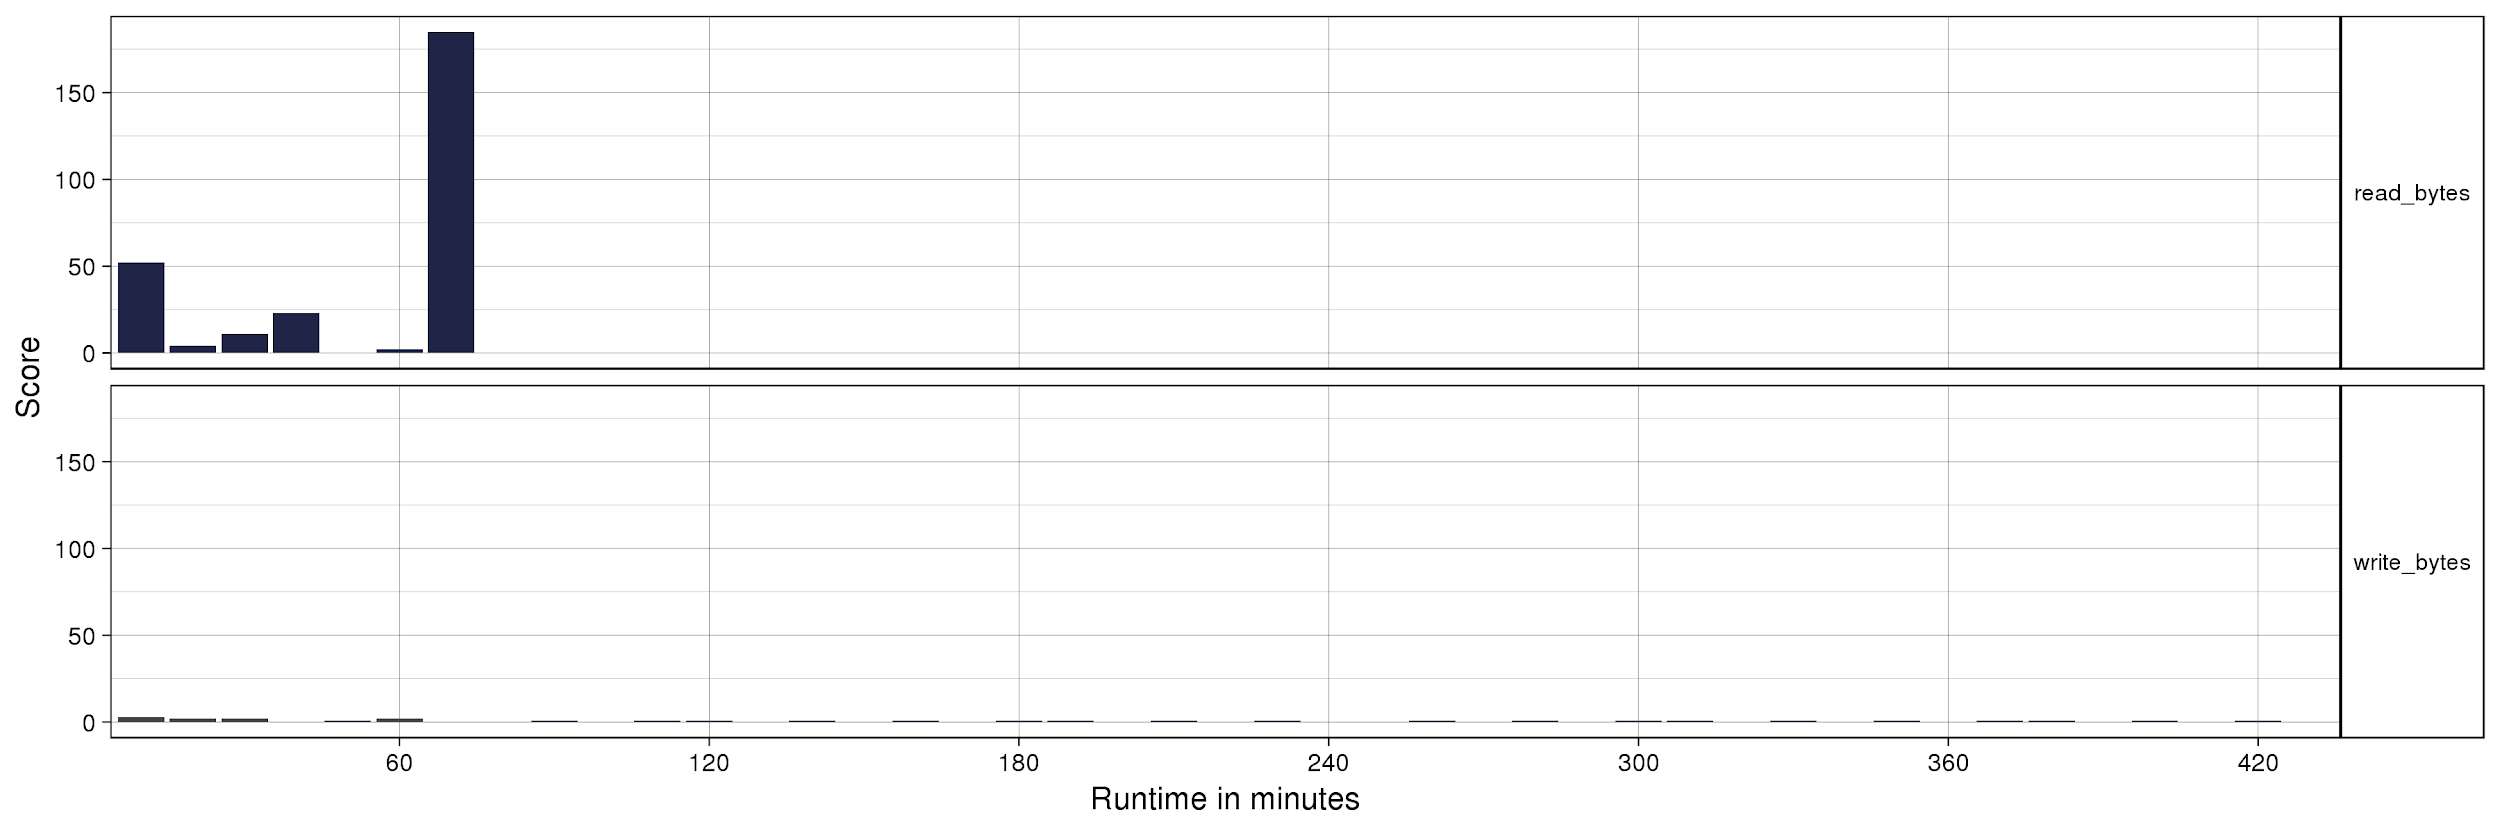
\includegraphics[width=4.61in,height=1.54in]{./media/image28.png}
	 \caption{Figure 3. Monitoring data of a 225 node job. Score is the sum of individual node scores.}
	 \label{fig:typ_io:2}
\end{figure}

\begin{figure}
	\centering
	 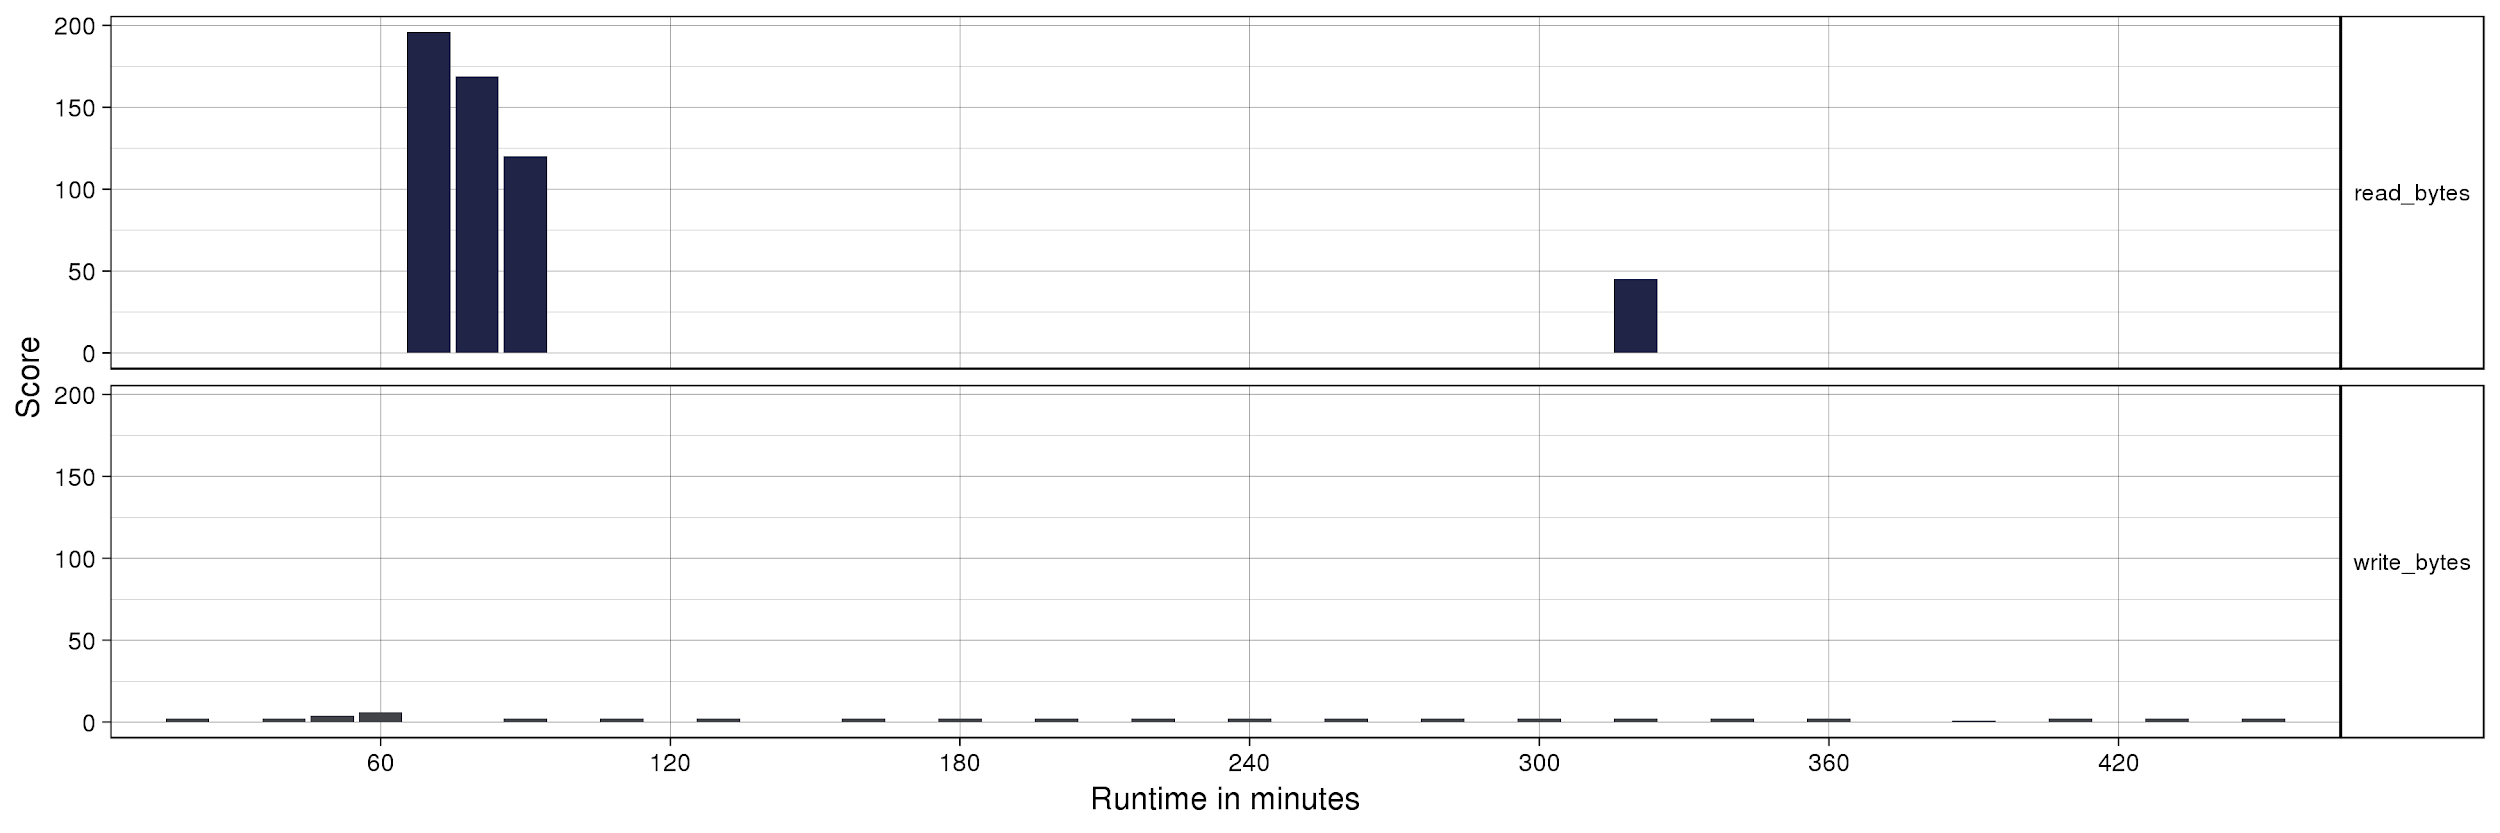
\includegraphics[width=4.61in,height=1.54in]{./media/image25.png}
	 \caption{Figure 4. Monitoring data of a 40 node job. Score is the sum of individual node scores.}
	 \label{fig:typ_io:3}
\end{figure}

Typical sources of variability when observing a performance metrics are: The concurrent usage of the shared storage, a shift between observed I/O phases due to network congestion or CPU throttling for power/heat reasons.
The same application using a different input configuration may need more compute time, resulting in longer phases between typical I/O patterns; moreover, it may change the I/O pattern.
A well-known pattern exhibited by a shorter running application may appear as well in a long-running application.
The similarity measure between two jobs should consider those sources of variability and allow us to provide a robust clustering of jobs depending on the user question.

There are different goals for the data analysis done by the user running the application or the support staff of the data center.
Whether or not the timeline is similar when executing an application with a different configuration and input dataset depends on the purpose of the analysis and task that follows the analysis.
For these reasons, we decided to explore a variety of alternative options for distance metrics and pre-processing and assess their suitability.


\section{Related work}
There are many tracing and profiling tools that are able to record I/O information~\cite{TFAPIKBBCF19}; we will discuss a selection of them in more detail in the following.
Most of them focus on individual jobs, and only a few of them apply machine learning for mass analysis.

The issue of performance profiles is that they remove the temporal dimension and make it difficult to identify relevant I/O phases.
As the purpose of interesting applications is the computation and I/O is just a byproduct, applications often spend less than 10\% time with I/O.
Tracing tools, however, produce too much information that must be reduced further.

The Ellexus tools\footnote{\url{https://www.ellexus.com/products/}} include Breeze, a user-friendly offline I/O profiling software, an automatic I/O report generator Healthcheck, and command line tool Mistral which purpose is to report on and resolve I/O performance issues when running complex Linux applications on high performance compute clusters.
Mistral is a small program that allows you to monitor application I/O patterns in real time, and log undesirable behaviour using rules defined in a configuration file called a contract.
Ellexus tools support POSIX and MPI (MPICH, MVAPICH, OpenMPI) I/O interfaces.

Darshan~\cite{carns2011understanding-toc,hpcdarshan} is an open source I/O characterization tool for post-mortem analysis of HPC applications' I/O behavior.
Its primary objective is to capture concise but useful information with minimal overhead.
Darshan accomplishes this by eschewing end-to-end tracing in favor of compact statistics such as elapsed time, access sizes, access patterns, and file names for each file opened by an application.
These statistics are captured in a bounded amount of memory per process as the application executes.
When the application shuts down, it is reduced, compressed, and stored in a unified log file.
Utilities included with Darshan can then be used to analyze, visualize, and summarize the Darshan log information.
Because of Darshan's low overhead, it is suitable for system-wide deployment on large-scale systems.
In this deployment model, Darshan can be used not just to investigate the I/O behavior of individual applications but also to capture a broad view of system workloads for use by facility operators and I/O researchers.

Darshan supports several types of instrumentation via software modules.
Each module provides its own statistical counters and function wrappers while sharing a common infrastructure for reduction, compression, and storage.
The most full-featured modules provide instrumentation for POSIX, MPI-I/O and standard I/O library function calls, while additional modules provide limited PNetCDF and HDF5 instrumentation.
Other modules collect system information, such as Blue Gene runtime system parameters or Lustre file system striping parameters.
The Darshan eXtended Tracing (DXT) module can be enabled at runtime to increase fidelity by recording a complete trace of all MPI-I/O and POSIX I/O operations.

Darshan uses LD\_PRELOAD to intercept I/O calls at runtime in dynamically linked executables and link-time wrappers to intercept I/O calls at compile time in statically linked executables.
For example, to override POSIX I/O calls, the GNU C Library is overloaded so that Darshan can intercept all the read, write and metadata operations.
In order to measure MPI I/O, the MPI libraries must be similarly overridden.
This technique allows an application to be traced without modification and with reasonably low overhead.

LASSi tool~\cite{DBLP:journals/corr/abs-1906-03884} was developed for detecting, the so called, victim and aggressor applications.
An aggressor can steal I/O resources from the victim and negatively affect its runtime.
To identify such applications, LASSi calculates metrics from Lustre job-stats and information from the job scheduler.
One metric category shows file system load and another category describes applications I/O behavior.
The correlation of these metrics can help to identify applications that cause the file system to slow down.
In the LASSi workflow this is a manual step, where a support team is involved in the identification of applications during file system slow down.
Manual steps are disadvantageous when processing large amounts of data and must be avoided in unsupervised I/O behavior identification.
LASSi's indicates that the main target group are system maintainers.
Understanding LASSi reports may be challenging for ordinary HPC users, who do not have knowledge about the underlying storage system.

The Nextgenio monitoring system~\cite{nextgenio2016}, has four main collectors.
The first two, the PBS and ALPS tools, collect job scheduling information.
The proprietary Cray I/O monitoring tool exploits Lustre I/O counters to capture file system usage on OSTs of all OSSs and allocated compute nodes.
The MAP component provides information about cpu, memory and network usage.
Then all the collected data is clustered for the analysis of system usage and performance evaluation.

In~\cite{TUISVPKB19}, the authors utilized probes to detect file system slow-down.
A probing tool measures file system response times by periodically sending metadata and read/write requests.
An increase of response times correlates to the overloading of the file system.
This approach allows the calculation of a slow-down factor identification of the slow-down time period.
This approach is able to detect a file system slow-down, but cannot detect the jobs that cause the slow-down.

\section{Methodology}
Generally, machine learning algorithms expect a fixed number of features.
As the number of time series  depends on the number of captured metrics, allocated nodes, and application runtime, this dynamic-sized monitoring data cannot be process directly.
Therefore, several post-processing steps must be applied from the raw time series and several choices must be made regarding the algorithmic processing using clustering algorithms.

To simplify the interpretation of results and the choice distance metrics, it is beneficial to have the same unit for all features which is why we use our category classification which creates a unitless order (see Section 2).
We also partition the data into segments of 10 minutes which we found previously is a good trade-off to represent the temporal behavior of the application while it reduces the size of the time series.
Hence, for a job and for each of our 9 client-side recorded metrics, we obtain a coarse-grained time series.
Each point represents a value across all nodes (such as mean, sum, or max) for the 10 minute interval.

In a \textbf{pre-processing} step, we extract a fixed number of features and compile them into what we call fingerprints.
A fingerprint represents a job's IO behavior.

Generally, deriving a fingerprint, can be done using one of the following approaches:


\begin{itemize}
	\item \textbf{Segment statistics} compute for each segment a fixed statistics, such as the mean value across all nodes.
		This basically preserves the time series and depends on the job-length.
	\item \textbf{Phase statistics} computes high-level statistics by analyzing the temporal behavior of IO phases further, e.g., compute the average length of IO segments with CriticalIO.
		This approach is independent of the job length but requires identifying phases and determining meaningful job metrics.
	\item \textbf{Job profiles} compute statistics across the whole job by eliminating the temporal component by applying reduction operations such as the arithmetic mean.
		A drawback of this simplification is that any temporal pattern is lost.
\end{itemize}

Once we picked the fingerprinting strategy, we must define a \textbf{similarity metric} between two fingerprints to allow clustering.
There are many possible choices that depend on the representation of the data.
If we consider fingerprints that are fixed size vectors such as for job profiles or phase statistics, then, e.g., cosine similarity or hamming distance can be applied.
If we aim to preserve the time series for segment statistics, then we can consider the vectors to be a string and, e.g., utilize the \textbf{Levenshtein distance} that counts the minimum number of modifications (inserts/deletes) between two strings.

Finally, the \textbf{clustering algorithm} needs to be selected.
Algorithms with a fixed number of clusters such as k-means, are not useful as the number of expressed job behaviors are unknown at the beginning.
Similarity clustering algorithms like DBSCAN or Agglomerative Clustering generate clusters depending on a user-chosen similarity value EPS.
Hierarchical clustering creates a hierarchy of jobs where similar jobs are linked closely together but suffer from quadratic runtimes.

In this paper, we explore the following combination of fingerprinting strategies and similarity metrics:

\begin{itemize}
	\item \textbf{Job profiles:} compute high-level statistics from the time series and apply a hierarchical clustering algorithm to group similar jobs automatically.
	\item \textbf{Segment statistics using Levenshtein distance:} convert segments into a time series of numbers and computes job similarity based on Levenshtein distance for all job pairs.
		\textbf{Phases matching:} extract phases from the segment statistics, finds best match between phases and computes job similarity for all job pairs.
\end{itemize}

Finally, we need to assess the quality of the obtained clusters.
Unfortunately, there are no tools that can do the cluster quality assessment automatically.
Therefore, we will inspect the clusters manually by using quantitative metrics such as the number of generated clusters and their sizes and qualitatively by exploring clusters of relevant jobs.
At this point we want to emphasize that our goal is to find similar jobs and not similar fingerprints.
Therefore, for the clustering quality assessment we look inside clusters and inspect segment sequences of the corresponding jobs.
In the same cluster we expect the sequences to be similar.
If not, clustering is not effective.

Depending on data, the clustering algorithms create thousands of clusters.
Unfortunately, it is not feasible to analyse all of them qualitatively with reasonable effort.
Therefore our analysis strategy is to find clusters with the characteristic weaknesses and discuss them.

\subsection{Overview}
In this work, we investigate several clustering algorithms for a large set of potential combinations of algorithms. The application of one algorithm can be understood as a number of successive processing steps on data. Roughly speaking, there are three basic steps: data pre-processing including coding, similarity computation, and clustering. In the following, we have dedicated a section to each step discussing potential alternatives. The list does not intend to be complete but shows a variety of options.

\subsubsection{Data pre-processing}
The 4-dimensional data from our monitoring system is to fine-grain mass analys. To be able to analyse millions of jobs, we apply some data reduction techniques that are listed in \Cref{tab:reduction_techniques}.
The result of the data-preprocessing is a coding of the initial time series data into one or multiple vectors.

\begin{table}
	\centering
	\begin{tabularx}{\textwidth}{llX}
		\hline
		Dimension       & Operation                                    &  Description                                                       \\ 
		\hline
		Time            &                                              &  Convert to various coding formats \par (see section 5.1.2 Coding) \\ 
		\hline
		Node            & Reduce by mean()                             &  Aggregate all nodes by mean() function                            \\ 
		\hline
		                & Reduce by sum()                              &  Aggregate all nodes by sum() function                             \\ 
		\hline
		File System     & Reduce by mean()                             &  Aggregate all file systems by mean() function                     \\ 
		\hline
		                & 
		Reduce by sum() & Aggregate all file systems by sum() function \\ 
		\hline
		Metric          & Reduce by sum()                              &  Aggregate all nine metrics by sum()                               \\ 
		\hline
		All             & Job profile                                  &  Reduces time series to a fixed set of values                      \\ 
		\hline
	\end{tabularx}
	\caption{Data reduction techniques.}
	\label{tab:reduction_techniques}
\end{table}


\subsubsection{Coding}
Segmented data can still contain too much information as necessary for the analysis.
To deal with that we introduce two further condensed data representations called binary and hexadecimal coding.
Additionally, we introduce two operations on codings.
One extracts I/O phases and the other one aggregates continuous zero segments to one zero segment.
The operations are summarized in \Cref{tab:coding_ops}.

\begin{table}
 \centering
 \begin{tabularx}{\textwidth}{lX}
	 \hline
	 Operation &  Description \\
	 \hline
	 Binarization & Segments are mapped to 9-bit numbers (v), where each position (i) represents a metric. The bits are set by the following function:
	 \vbox{
		\begin{equation}
			v_i = 
			\begin{cases}
				\text{false if segment}_i = 0\\\text{true otherwise.}
			\end{cases}, i \in [\text{enumerated metrics}]
		\end{equation}
	 } \\
	 \hline
	 Hex-Quantization & Quantize segments to 16 levels. \\
	 \hline
	 Zeros aggregation & Aggregates continuous occurrences of zero segments to one zero segment. \\
	 \hline
	 Phase extraction &  Extract continuous sequences of non-zero segments. \par - Splits time series at zero segments in sub time series (I/O phases) and removes zero segments. \par - Preserves order of I/O phases. \\
	 \hline
 \end{tabularx}
 \caption{Coding operations.}
 \label{tab:coding_ops}
\end{table}


\paragraph{Binary coding}
Binary coding represents monitoring data as a sequence of numbers, where each number stands for a kind of file system usage.
The number depends on activities found in the segment.
In this coding approach each conceivable combination of activities has an unique number.

The approach maps the three categories to the following two states: The LowIO category is mapped to the non-active (0) state, and HighIO and CriticalIO categories are mapped to the active (1) state.
On one side, by doing this, we lose information about performance intensity, but on other side, this simplification allows a more comprehensible comparison of job activities.

In our implementation, we use a 9-bit number to represent each segment, where each bit represents a metric.
The bit is 1 if the corresponding metric is active, and 0 if not.
Translated to the decimal representation, metric segments can be coded as 1, 2, 4, 8, 16, and so on.
%\textcolor[HTML]{1155CC}{\uline{Table 5}} shows codings used in this work.

Using this kind of coding we can compute a number for each segment, that describes unambiguously the file system usage, e.g., a situation where intensive usage of md\_read (Code=16) and read\_bytes (Code=32) occur at the same time and no other significant loads are registered is coded by the value 48.
Coding is reversible, e.g., when having value 48, the computation of active metrics is straightforward.

%%%%%%%%%%%%%%%%%%%%% Table No: 3 starts here %%%%%%%%%%%%%%%%%%%%


%\begin{table}[H]
%       \centering
%\begin{tabular}{p{0.8in}p{0.8in}}
%\hline
%%row no:1
%\multicolumn{1}{p{0.8in}}{\cellcolor[HTML]{C9DAF8} \tabto{0.25in}  \tabto{0.39in} \tab Metric} & 
%\multicolumn{1}{p{0.8in}}{\cellcolor[HTML]{C9DAF8} \tabto{0.25in}  \tabto{0.39in} \tab Code} \\
%\hhline{--}
%%row no:2
%\multicolumn{1}{p{0.8in}}{md\_file\_create} & 
%\multicolumn{1}{p{0.8in}}{ \tabto{0.25in}  \tabto{0.39in} \tab 1} \\
%\hhline{~~}
%%row no:3
%\multicolumn{1}{p{0.8in}}{md\_file\_delete} & 
%\multicolumn{1}{p{0.8in}}{ \tabto{0.25in}  \tabto{0.39in} \tab 2} \\
%\hhline{~~}
%%row no:4
%\multicolumn{1}{p{0.8in}}{md\_mod} & 
%\multicolumn{1}{p{0.8in}}{ \tabto{0.25in}  \tabto{0.39in} \tab 4} \\
%\hhline{~~}
%%row no:5
%\multicolumn{1}{p{0.8in}}{md\_other} & 
%\multicolumn{1}{p{0.8in}}{ \tabto{0.25in}  \tabto{0.39in} \tab 8} \\
%\hhline{~~}
%%row no:6
%\multicolumn{1}{p{0.8in}}{md\_read} & 
%\multicolumn{1}{p{0.8in}}{ \tabto{0.25in}  \tabto{0.39in} \tab 16} \\
%\hhline{~~}
%%row no:7
%\multicolumn{1}{p{0.8in}}{read\_bytes} & 
%\multicolumn{1}{p{0.8in}}{ \tabto{0.25in}  \tabto{0.39in} \tab 32} \\
%\hhline{~~}
%%row no:8
%\multicolumn{1}{p{0.8in}}{read\_calls} & 
%\multicolumn{1}{p{0.8in}}{ \tabto{0.25in}  \tabto{0.39in} \tab 64} \\
%\hhline{~~}
%%row no:9
%\multicolumn{1}{p{0.8in}}{write\_bytes} & 
%\multicolumn{1}{p{0.8in}}{ \tabto{0.25in}  \tabto{0.39in} \tab 128} \\
%\hhline{~~}
%%row no:10
%\multicolumn{1}{p{0.8in}}{write\_calls} & 
%\multicolumn{1}{p{0.8in}}{ \tabto{0.25in}  \tabto{0.39in} \tab 256} \\
%\hhline{~~}

%\end{tabular}
% \end{table}


%%%%%%%%%%%%%%%%%%%%% Table No: 3 ends here %%%%%%%%%%%%%%%%%%%%

%\begin{Center}
%Table 5. Metric codes 
%\end{Center}


To reduce the 4-dimensional data, we reduce that structure to two dimensions (segments metrics) by aggregating other dimensions by applying sum() function on score values.
In the resulting table we leave zero scores, and change scores larger than zero to one.


After coding each segment, the jobs can be represented as a sequence of numbers, e.g.,

\begin{lstlisting}
'jobid': 'jobA', 'coding': [1:5:0:0:0:0:0:0:96:96:96:96:96:96:96], 'length': 15
\end{lstlisting}


The monitoring dataset doesn't provide information about what happens during the zero segments.
It can be anything, like a job is waiting for resources, or computing something.
It can also be that the job script cannot start immediately or run on a slow network.
To catch such jobs, we aggregate multiple consecutive zero segments into one zero segment, thus the coding of the previous job would be:


\begin{lstlisting}
'jobid': 'jobA', 'coding': [1:5:0:96:96:96:96:96:96:96], 'length': 15
\end{lstlisting}

Note, that the job length does not change, only the sequence length.

\paragraph*{Hexadecimal coding}
Hexadecimal coding preserves monitoring data for each metric and each segment.
As the name suggests, a segment is converted into a hexadecimal number.
The numbers are obtained in two steps.
Firstly, the dimension reduction aggregates the file system and the node dimensions and computes a mean value for each metric and segment, which lies in interval [0,4].
Secondly, the mean values are quantized into 16 levels -- 0 represents the interval [0,0.125), 1 [0.125,0.375), $ \ldots $ , f [3.625, 4].
The example in \Cref{tab:hex_example} shows hexadecimal coding for a job containing 6 segments.

\begin{table}
  \centering
  \begin{tabular}{ll}
    md\_file\_create & [0:0:\textbf{2}:\textbf{2}:\textbf{2}:\textbf{9}] \\ 
    md\_file\_delete & [0:0:0:0:0:0]                                     \\ 
    md\_mod          & [0:0:0:0:0:0]                                     \\ 
    md\_other        & [0:0:0:0:0:0]                                     \\ 
    md\_read         & [0:0:0:\textbf{9}:3:0]                            \\ 
    read\_bytes      & [\textbf{5}:0:0:0:0:0]                            \\ 
    read\_calls      & [0:0:0:0:0:0]                                     \\ 
    write\_bytes     & [0:0:0:0:\textbf{f}:\textbf{f}]                   \\ 
    write\_calls     & [0:0:0:0:0:0]
  \end{tabular}
  \caption{Example of a hexadecimal coding.}
  \label{tab:hex_example}
\end{table}

\subsubsection{Similarity}
Determining the resemblance between two jobs is the main task of this work.
We developed a couple of strategies to do that task.
They are listed in \Cref{tab:sim_funcs}.
As we will see later, under some circumstances they can be used together in one clustering stack.

\begin{table}
  \centering
	\begin{tabularx}{\textwidth}{lX}
    \hline
    Operation & Description \\
    \hline
    Euclidean & \\
    \hline
    Levenshtein &  - Number of operation (inserts, deletes, and changes) requires to convert one coding in another \\
    \hline
    Sliding window &  - Find maximum similarity between two codings \par - Slide shorter coding over a longer one an compute similarity of the corresponding parts \\
    \hline
    Phase &  - Find best I/O phases combination of two jobs with a maximum similarity \par - Depends on phase extraction from data pre-processing and sliding window similarity \par - Preserve the order of the phases \\
    \hline
  \end{tabularx}
  \caption{Similarity functions}
  \label{tab:sim_funcs}
\end{table}

\subsubsection{Clustering}
In the last step, similar jobs need to be grouped in clusters.
To handle millions of jobs, the algorithm must be performant.
We developed two strategies that meet the requirement, one based on widely used general-purpose algorithms, and a custom algorithm.
They are listed in \Cref{tab:clustering_algorithms}.
For scalability reasons, we derived two algorithms that are able to handle the large number of jobs but aim to preserve the core ideas of existing algorithms.

\begin{table}
  \centering
  %\begin{tabular}{p{0.99in}p{3.2in}}
	\begin{tabularx}{\textwidth}{lX}
    \hline
    Algorithm & Description \\
    \hline
    Random & k-means picks random \\
    \hline
    Density clustering &  DBSCAN $ \ldots $  is equal or larger than the user defined value. \\
    \hline
    Agglomerative &  Hierarchical clustering \\
    \hline
    ClusteringTree &  Applies ideas from hierarchical clustering using a decision tree. \\
    \hline
    SimplifiedDensity &  Combines ideas from k-means with density clustering. The simplified clustering algorithms add a job to a cluster if similarity to the cluster centroid is equal or larger than the user defined value. \\
    \hline
  \end{tabularx}
  \caption{Clustering algorithms}
  \label{tab:clustering_algorithms}
\end{table}


\paragraph{ClusteringTree algorithm}
This algorithm involves three steps:

\begin{enumerate}
 \item Agglomerative clustering of small dataset
 \item Training of a decision tree model
 \item Clustering with the decision tree
\end{enumerate}

%\eb{(Move generic stuff up here from below or write that details are described below).}

\paragraph{SimplifiedDensity algorithm}
Clusters are formed around centroids.
That are job codings that form clusters by attracting similar jobs.
All jobs in a cluster fulfill only one condition, the similarity (SIM) to the centroid has to be larger than the user defined minimum.
The jobs are put in the first cluster, where the condition is fulfilled.
If there is no such a cluster, the job forms a new one.

These low requirements allow a performant implementation, but they also allow a job to be in one cluster, even if a centroid of another cluster is much closer, as long as the condition is true.
The result depends on the processing order of the jobs, though but it is deterministic.

The algorithm can be summarized as follows.

\begin{enumerate}
 \item Pick one arbitrary job from the dataset, which will serve as a cluster centroid, and compute similarity to all other jobs.
 \item Create a cluster of jobs that have a minimum similarity and remove them from the dataset.
 \item Repeat step 1 and 2 until no jobs are left in the dataset.
\end{enumerate}

\subsubsection{Clustering stacks}
There are several combinations possible.
In this work, we investigate six of them.
The operation stack used in each is visualized \Cref{fig:clustering_stacks}.

\begin{figure}
  \centering
  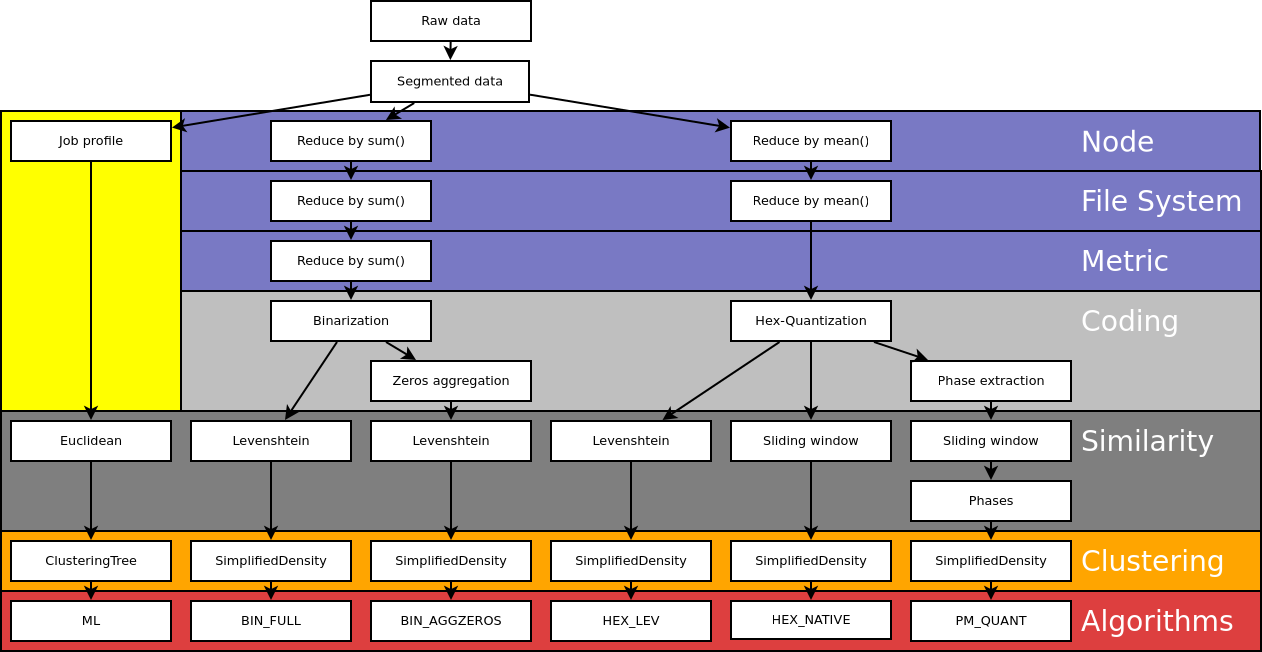
\includegraphics[width=4.61in,height=2.38in]{./media/image3.png}
  \caption{Algorithms and their actual clustering stacks.}
  \label{fig:clustering_stacks}
\end{figure}

\begin{itemize}
 \item Approach 1 (ML) uses a set of\textbf{ traditional machine learning} techniques. 
 \item Approach 2 (BIN\_ALL): \textbf{Levenshtein} distance on \textbf{binary codings.}
 \item Approach 3 (BIN\_AGGZEROS) is like BIN\_ALL, but with \textbf{zero aggregation }of contiguous zero segments.
 \item Approach 4 (HEX\_LEV): Experiments with \textbf{hexadecimal coding }and \textbf{Levenshtein }distance.
 \item Approach 5 (HEX\_NATIVE): is like HEX\_LEV, but uses a \textbf{performance-aware }similarity function.
 \item Approach 6 (PM\_QUANT) is like HEX\_NATIVE, but uses a \textbf{phase-aware }similarity function.
\end{itemize}

During our research, we explored various additional combinations: (kurze Liste), but we found that these do not perform well and are not interesting to discuss.

\subsection{Algorithms }
\subsubsection{ML general-purpose machine learning algorithms}
In the preprocessing step, the MinMaxScaler scales the features are scaled to values between 0 and 1 using MinMax normalization.
Therefore, the highest distance between two points can be at most EPS\_MAX =  \( d^{1/d} \) , where d is the dimension of the dataset.


The agglomerative clustering algorithm uses euclidean distance as a similarity measure, i.e., if the distance between two points is shorter than a maximum distance (EPS), then these points belong to the same cluster.
We explore several EPS between 0 and EPS\_MAX and use the best value for further evaluation.


The application of general-purpose machine learning algorithms on fingerprints of data is simple.
With little effort, the fixed-size fingerprints can be transformed into the fixed size input format accepted by the algorithm, but we find quickly that the size of our datasets is the first obstacle to the suitable clustering algorithms.
For example, the scaling behaviour of the agglomerative clustering algorithm that is used in this work can handle around 10,000 jobs in a reasonable amount of time as the complexity is  \( N^{2} \) .
Nevertheless, with a workaround, which involves additional classification steps, we are able cluster 1,000,000 samples.
This workaround involves three steps.

\begin{enumerate}
 \item Clustering and labeling 10,000 jobs with agglomerative clustering algorithm
 \item Training of a decision tree model with data from the previous step
 \item Predict labels of 1,000,000 jobs with the trained decision tree model
\end{enumerate}

\subsubsection{BIN\_ALL}
The Levenshtein based similarity between two jobs can be determined by the following formula.
It is the number of Levenshtein operations (changes/deletes/inserts) divided by the length of the longest sequence, and subtracted from the value one.
This function works with binary coding.

\begin{equation}
similarity \left( job_{A}\text{, jo}b_{B} \right) =1- \frac{levenshtein \left( coding_{A}\text{, codin}g_{B} \right) }{max \left( length_{A}\text{, lengt}h_{B} \right) }
\end{equation}

\begin{lstlisting}
{'jobid': 'jobA',
'coding': [1:5:0:0:0:0:0:0:96:96:96:96:96:96:96],
'length': 15} 

{'jobid': 'jobB',
'coding': [0:0:0:0:0:0:0:0:0:96:96:96:96:96:98],
'length': 15}
\end{lstlisting}

The similarity between these two jobs according to this equation is 73 percent.

\subsubsection{BIN\_AGGZEROS}
As a variation we investigated also the case where the the zero-sequences in are reduced to a single zero segment. This allow us to focus on I/O intensive parts of the job. The example below shows reduced codings from the previous example. Note, that the job did not change.

\begin{equation}
similarity \left( job_{A}\text{, jo}b_{B} \right) =1- \frac{levenshtein \left( coding_{A}\text{, codin}g_{B} \right) }{max \left( length_{A}\text{, lengt}h_{B} \right) }
\end{equation}

\begin{lstlisting}
{'jobid': 'jobA',
'coding': [1:5:0:96:96:96:96:96:96:96],
'length': 15}

{'jobid': 'jobB',
'coding': [0:96:96:96:96:96:98],
'length': 15}
\end{lstlisting}

The computation of similarity do not change.
For this coding it is 53 percent.


\subsubsection{HEX\_LEV}
This similarity function works on the same principle like the BIN functions, with the difference that it computes the similarity for all metrics, and then the mean value of the similarities.
This adaption allows to apply Levenshtein-based similarity on hexadecimal coding.

\begin{align}
  similarity \left( job_{A}\text{, jo}b_{B} \right) &= 1 -\frac{ \sum_{m \in Metric}^{} levenshtein \left( coding_{A,m}\text{, coding}_{B,m} \right) }{N \cdot L_{B}} \\
	&\text{, with }L_{B} \geq L_{A}
\end{align}

\subsubsection{HEX\_NATIVE}
The similarity function below computes a performance aware similarity between two jobs.
It works with hexadecimal codings at metric level, i.e., it computes maximum similarity between metrics and computes a mean value of them.
Assume jobB is larger or equal than jobA, the job similarity between two jobs can be computed by the following equation.

\begin{align}
similarity \left( job_{A}\text{, jo}b_{B} \right) &= 1-\frac{ \sum _{m \in Metric}^{}maxCodingSimilarity \left( job_{A,m}\text{, jo}b_{B,m} \right) }{L_{B}}\\
&\text{, with }L_{B} \geq L_{A}
\end{align}

The metric coding sequences $job_{B,m}$ and $job_{A,m}$ of different jobs can have different lengths.
Therefore, to compute a maximum similarity between two metrics, we use a sliding window approach.
That means, we take the shortest coding sequence (CA) and slice the longest coding sequence (CB) in slices of the same length, and compute the similarities between them, as shown in the pseudo code below.

\begin{lstlisting}
float maxCodingSimilarity(CA, CB) { 
  max = 0
  LA = length(CA)
  LB = length(CB)
  for pos in 0..(LB-LA) { // LB-LA is the boundary, as stated: LB > LA
    sim = sliceSimilarity(CA, substr(str=CB, start=pos, len=LA))
    if sim > max {
      max = sim
    }
  }
  return max
}
\end{lstlisting}

The sliceSimilarity() computes similarity between two codings of the same length.
This function maps the difference between performance levels of the same segments (values between 0 and 16) to a relative value between 0 and 1.

\begin{equation}
sliceSimilarity \left( S_{A},S_{B} \right) =\frac{ \sum _{i=1}^{L_{}}16 - \vert S_{A,i}-S_{B,i} \vert }{\text{16 L}_{}}\text{, with }L=L_{B}=L_{A}
\end{equation}

\subsubsection{PM\_QUANT}
There is a lack of clustering algorithms that can cluster variable length arrays or words.
We developed a clustering strategy tailored to the IO phases.

\paragraph{Hexadecimal coding}
Suppose there are hexadecimal codings of two jobs with different lengths.
In the example below bold\ font emphasizes I/O intensive  metrics and red colored numbers emphasize I/O intensive metric segments.


\begin{lstlisting}
{ 
'jobid': jobA,
'coding': metric
md_file_create [0:0:2:2:2:9:3:0:9:1:1:1:0]
md_file_delete [0:0:0:0:0:0:0:0:0:0:0:0:0]
md_mod         [0:0:0:0:0:0:0:0:0:0:0:0:0]
md_other       [0:0:0:0:0:0:0:0:0:0:0:0:0]
md_read        [0:0:0:9:3:0:0:0:0:0:1:0:0]
read_bytes     [0:0:0:0:0:0:0:0:0:0:0:0:0]
read_calls     [0:0:0:0:0:0:0:0:0:0:0:0:0]
write_bytes    [0:0:0:0:0:0:0:0:0:0:0:0:0]
write_calls    [0:0:0:0:0:0:0:0:0:0:0:0:0]
'length': 13} 

{ 
'jobid': jobB,
'coding': metric
md_file_create [1:0:0:0:0:0:0:0:0:0:0:0:0:0:0]
md_file_delete [0:0:0:0:0:0:0:0:0:0:0:0:0:0:0]
md_mod         [0:0:0:0:0:0:0:0:0:0:0:0:0:0:0]
md_other       [0:0:0:0:0:0:0:0:0:0:0:0:0:0:0]
md_read        [0:0:0:0:0:0:0:0:0:0:0:0:0:0:0]
read_bytes     [2:2:2:2:8:2:2:0:0:1:0:0:8:1:1]
read_calls     [0:0:0:0:0:0:0:0:0:0:0:0:0:0:0]
write_bytes    [0:0:0:0:0:0:0:0:0:0:0:5:0:0:0]
write_calls    [0:0:0:0:0:0:0:0:0:0:0:0:0:0:0]
'length': 15} 
\end{lstlisting}

\paragraph{Phase detection}
According to our I/O phase definition, phases are separated by zeros.
This definition makes the detection of individual phases to a trivial task.
Relevant for similarity computation are only metrics that contain at least one non-zero segment.
In this example, that is md\_file\_create, read\_bytes and write\_bytes metrics.
The according phases are illustrated below.

\begin{lstlisting}
job_1_md_file_create : [[2,2,2,9,3], [9,1,1,1]]
job_1_read_bytes : [[9,3], [1]]
job_1_write_bytes : []

job_2_md_file_create : [[1]]
job_2_read_bytes : [[2,2,2,2,8,2,2], [1], [8,1,1]]
job_2_write_bytes : [[5]]
\end{lstlisting}


\paragraph{Phase matching}
Sliding the shorter coding over a longer one, and computing similarity to the corresponding part, we can find the best match.
The example below illustrates that.
We find the best match, when we the shift shorter coding five position to the right.


\noindent\begin{minipage}{0.33\textwidth}
\begin{lstlisting}
[2:2:2:2:8:2:2]
[9:3:-:-:-:-:-]
similarity 
= (2/9+2/3)/7 
= 13%

[2:2:2:2:8:2:2]
[-:9:3:-:-:-:-]
similarity 
= (2/9+2/3)/7 
= 13%
\end{lstlisting}
\end{minipage}
%
\begin{minipage}{0.33\textwidth}
\begin{lstlisting}
[2:2:2:2:8:2:2]
[-:-:9:3:-:-:-]
similarity 
= (2/9+2/3)/7 
= 13%

[2:2:2:2:8:2:2]
[-:-:-:9:3:-:-]
similarity 
= (2/9+3/8)/7
= 8%
\end{lstlisting}
\end{minipage}
%
\noindent\begin{minipage}{0.33\textwidth}
\begin{lstlisting}
[2:2:2:2:8:2:2]
[-:-:-:-:9:3:-]
similarity
= (8/9+2/3)/7
= 22%

[2:2:2:2:8:2:2]
[-:-:-:-:-:9:3]
similarity 
= (2/9+2/3)/7 
= 13%
\end{lstlisting}
\end{minipage}


After repeating this step for all possible combinations of I/O phases we chose those with the pairs with the highest similarity, and compute match between them.
To compute the match we divide low hex value by high hex value for each segment and sum up the values.
I/O phases without a pair are assigned virtually to empty phases, and their match is zero.
The example below shows I/O phases pairs and their matches.

\begin{lstlisting}
job1_md_file_create : [[2:2:2:9:3], [9:1:1:1]]
job2_md_file_create : [[-:-:-:-:-], [-:1:-:-]]
match_md_file_create = [(match:0; len:5), (match:1; len:4)]
 
job1_read_bytes : [[-:-:-:-:9:3:-], [1], [-:-:-]]
job2_read_bytes : [[2:2:2:2:8:2:2], [1], [8:1:1]]
match_read_bytes = [match:(8/9 + 2/3); len:7), (match:1; len:1), (match:0; len:3)]

job1_write_bytes = [[-]]
job2_write_bytes = [[5]]
match_write_bytes = [(match:0; len:1)]
\end{lstlisting}

\paragraph{Similarity}

Next, the similarity for coding with different lengths must be adjusted. Similarity between two jobs is the sum of matches divided by the sum of lengths of the longer phases. In this example, we get a similarity of 17$\%$ .

similarity = (0 + 1 + 8/9 + 2/3 + 1 + 0 + 1) / (5 + 4 + 1 + 7 + 3 + 1) = 0.17

\subsection{Data}
From the perspective of this work, analysis of non-I/O-intensive jobs (zero-jobs) has no advantage.
On the contrary, they could hide some interesting aspects for the BIN and HEX algorithms.
For example, these algorithms would distribute them across different clusters, instead of placing them in one cluster.
For that reason, we detect zero-jobs early and remove them from datasets.
By the way, PM ignores such jobs by design.
Therefore, this step wouldn't be necessary.

The\ number of zero-jobs is different for hexadecimal and absolute mode codings.
The reason is the quantization to HEX coding, which firstly computes mean performance values for all segments, and then quantizes them to 16 levels.
Hereby some segments can be quantized to zeros, if the mean value becomes sufficiently low.
Therefore, it may happen that some jobs fall into the zero-job category, if all segments are quantized to zeros.
 It can not happen in BIN coding, because it preserves all the active segments, so that no job may change the category.
Interestingly, it affects around 14$\%$  of jobs.
\Cref{tab:n_intensive_jobs} shows the number of jobs that are used for clustering algorithms.

\begin{table}
  \centering
  \begin{tabular}{ll}
    \hline
    Algorithm & Number of I/O intensive jobs \\
    \hline
    BIN\_$\ast$, PM\_FLOAT, HEX\_NATIVE &  583.000 \\
    \hline
    HEX\_LEV, PM\_QUANT &  444.000 \\
    \hline
  \end{tabular}
  \caption{Numbers of I/O-intensive jobs.}
  \label{tab:n_intensive_jobs}
\end{table}

\subsubsection{Data exploration}
I/O phases are, according to our definition, contiguous sequences of I/O intensive segments.
The corresponding statistics are visualized in \Cref{fig:phases_stats}.
We suppose this characteristic can be exploited in clustering algorithms to achieve better results.

\begin{figure}
  \centering
  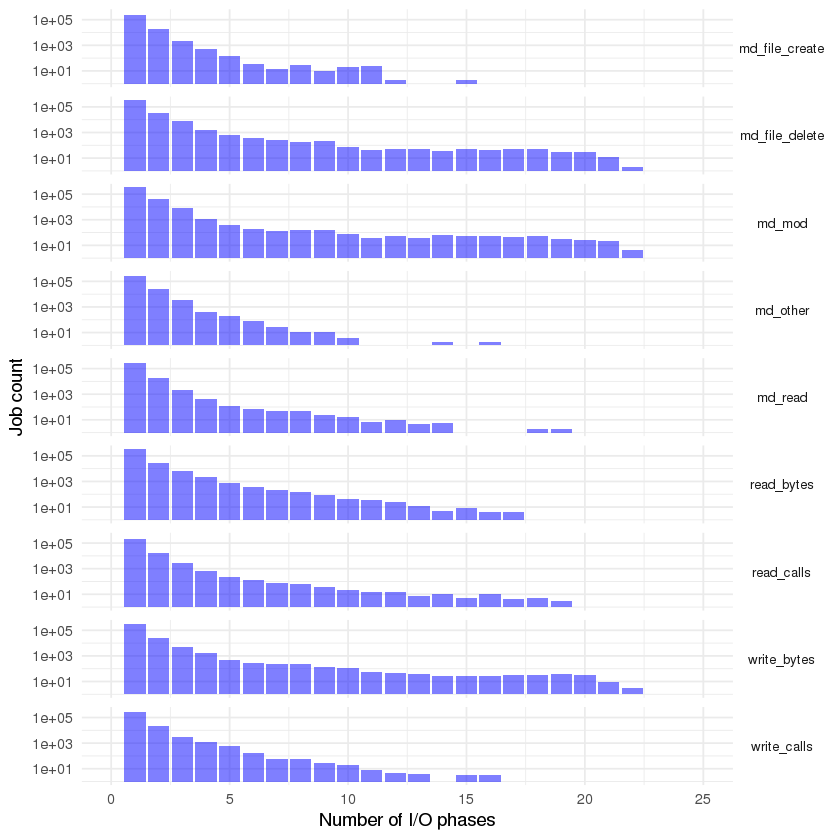
\includegraphics[width=3.55in,height=3.56in]{./media/image23.png}
  \caption{I/O phases statistics.}
  \label{fig:phases_stats}
\end{figure}

\subsection{Evaluation of general-purpose clustering algorithms}
This section contains data statistics, and the clustering results in \Cref{fig:datasets_clustering_results} of the Job-IO-Metric and Job-IO-Duration datasets with general-purpose machine learning algorithms.
Due to lack of tools, we determine cluster quality on a small scale.

\subsubsection{Test environment}
All the experiments in this section are conducted with python 3.8.0.
In particular we use the agglomerative clustering algorithm, decision trees, and the MinMaxScaler from the sklearn 0.22.1 library.

\begin{figure}
	\begin{subfigure}[t]{0.45\textwidth}
	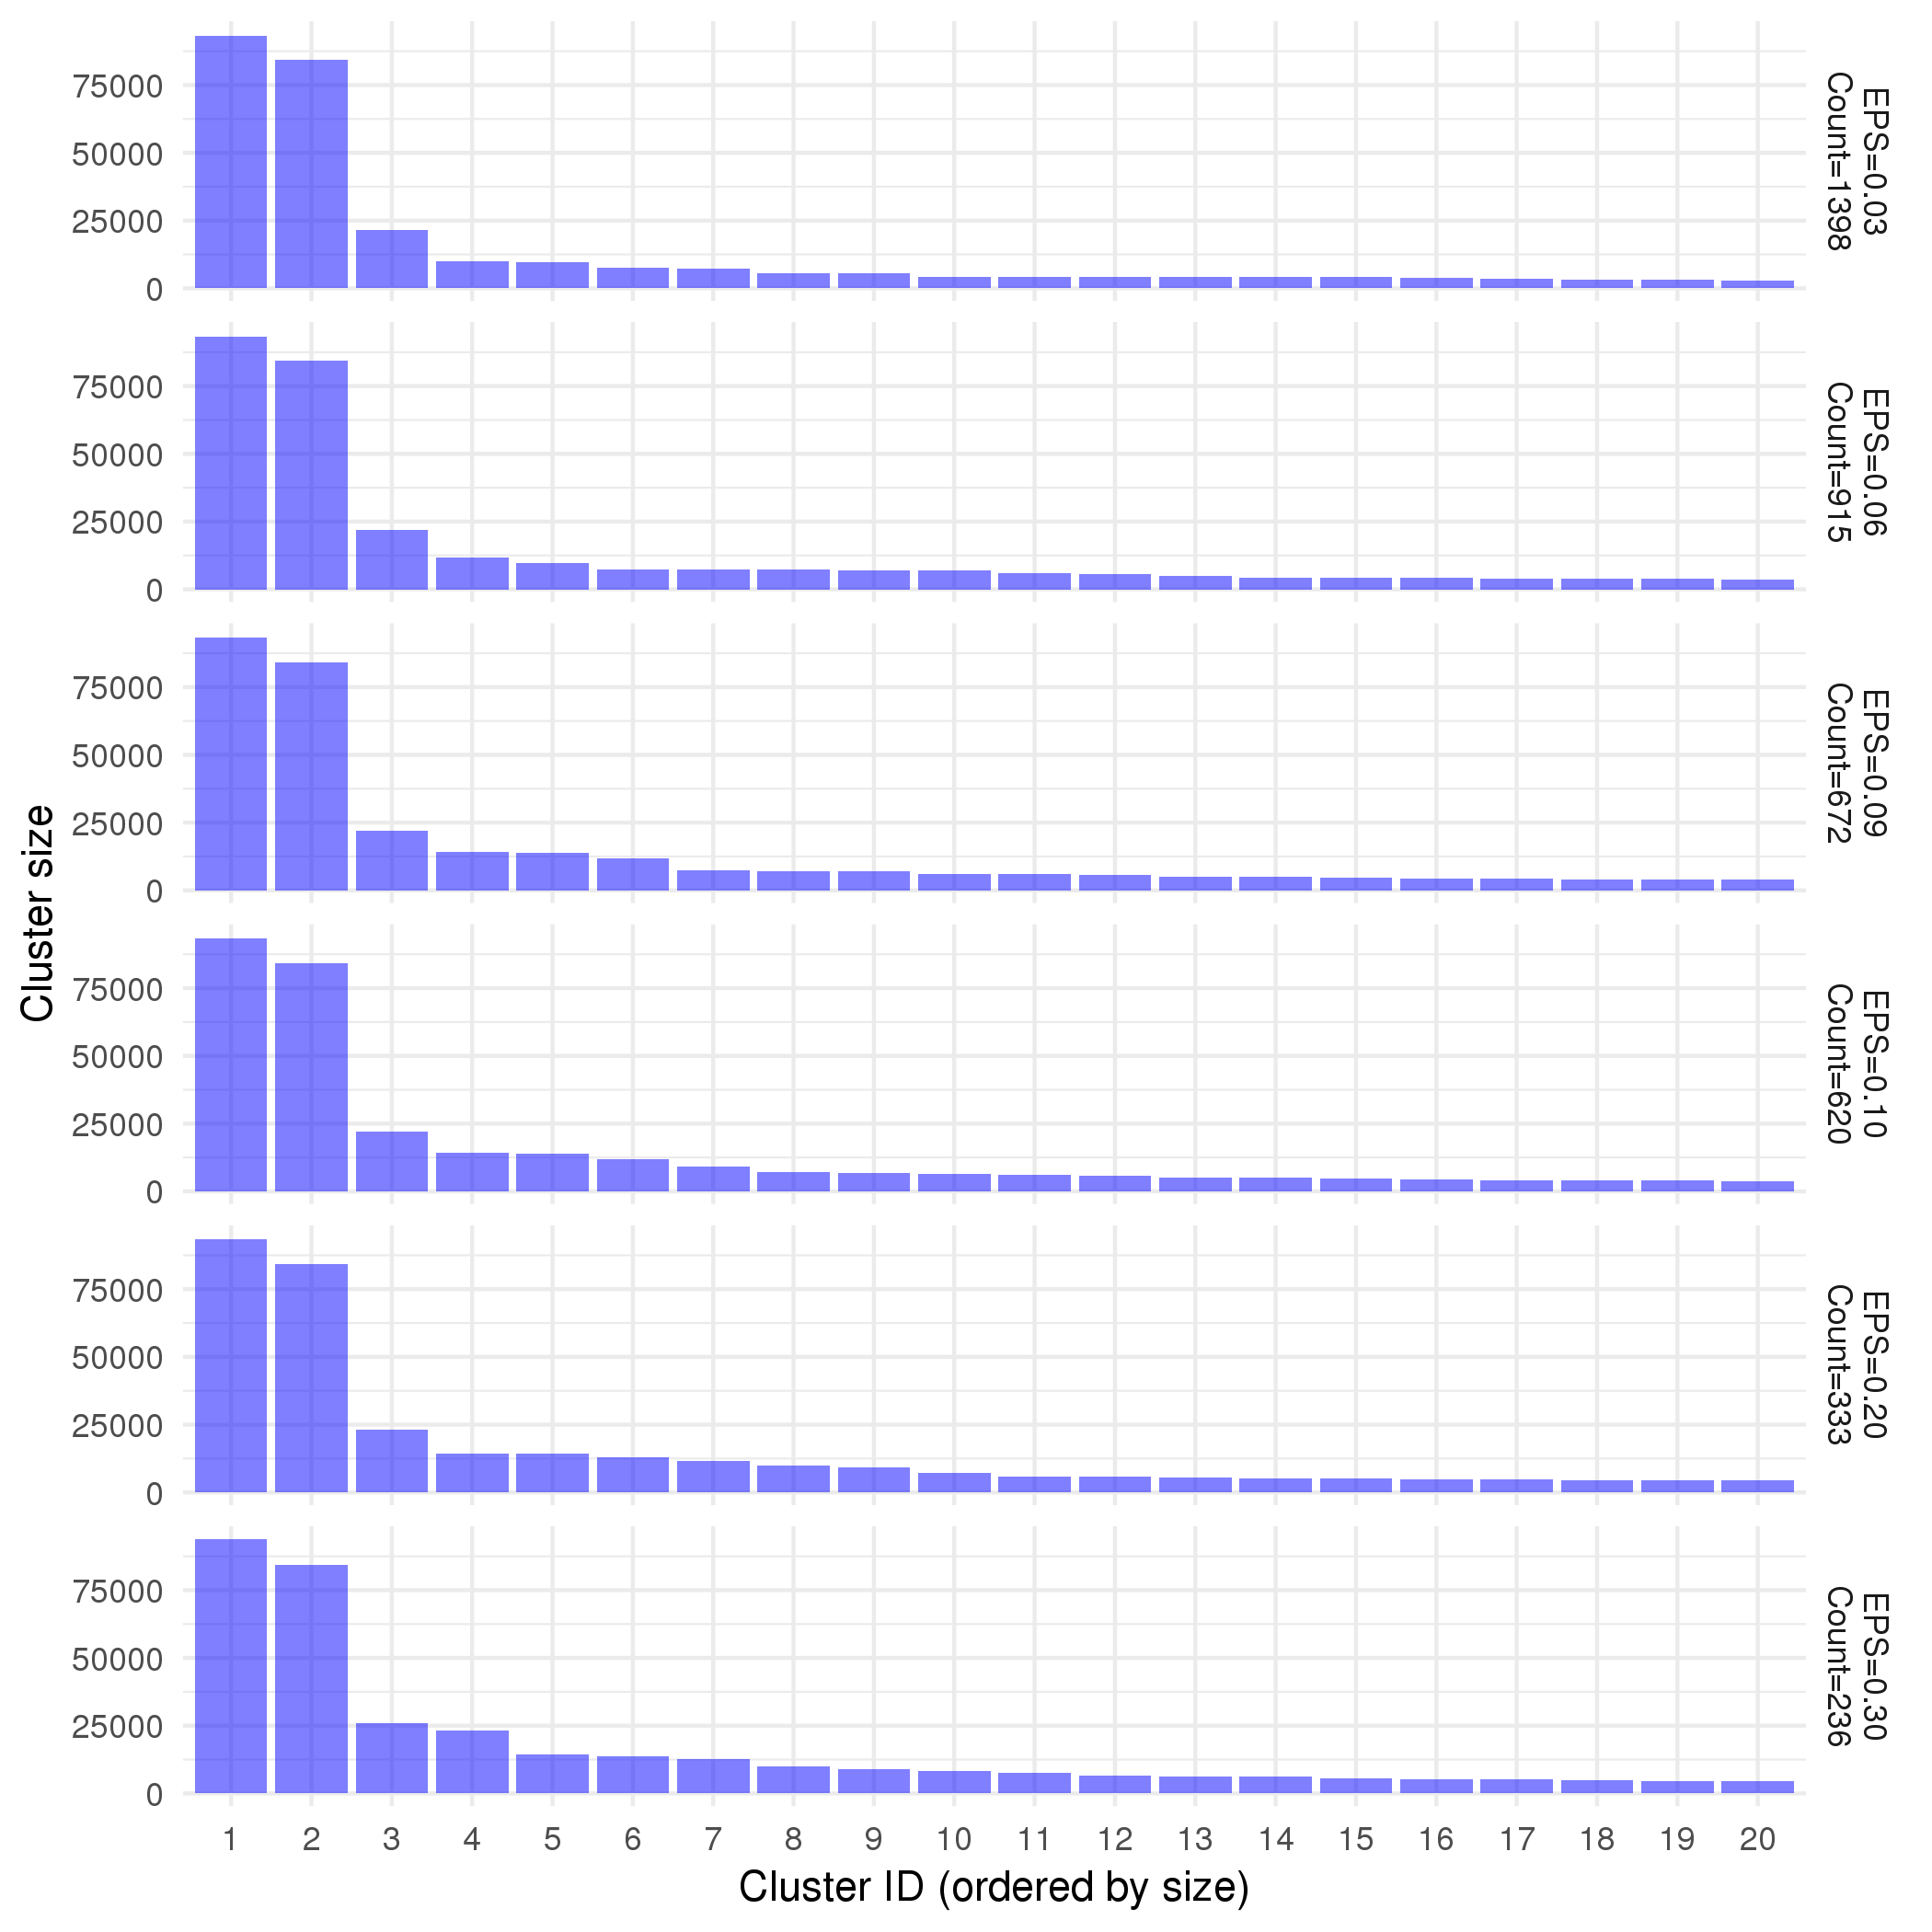
\includegraphics[width=\textwidth]{./media/image10.png}
	\caption{Job-IO-Duration}
	\label{fig:datasets_clustering_results:io_duration}
 \end{subfigure}
 \hfill
 \begin{subfigure}[t]{0.45\textwidth}
	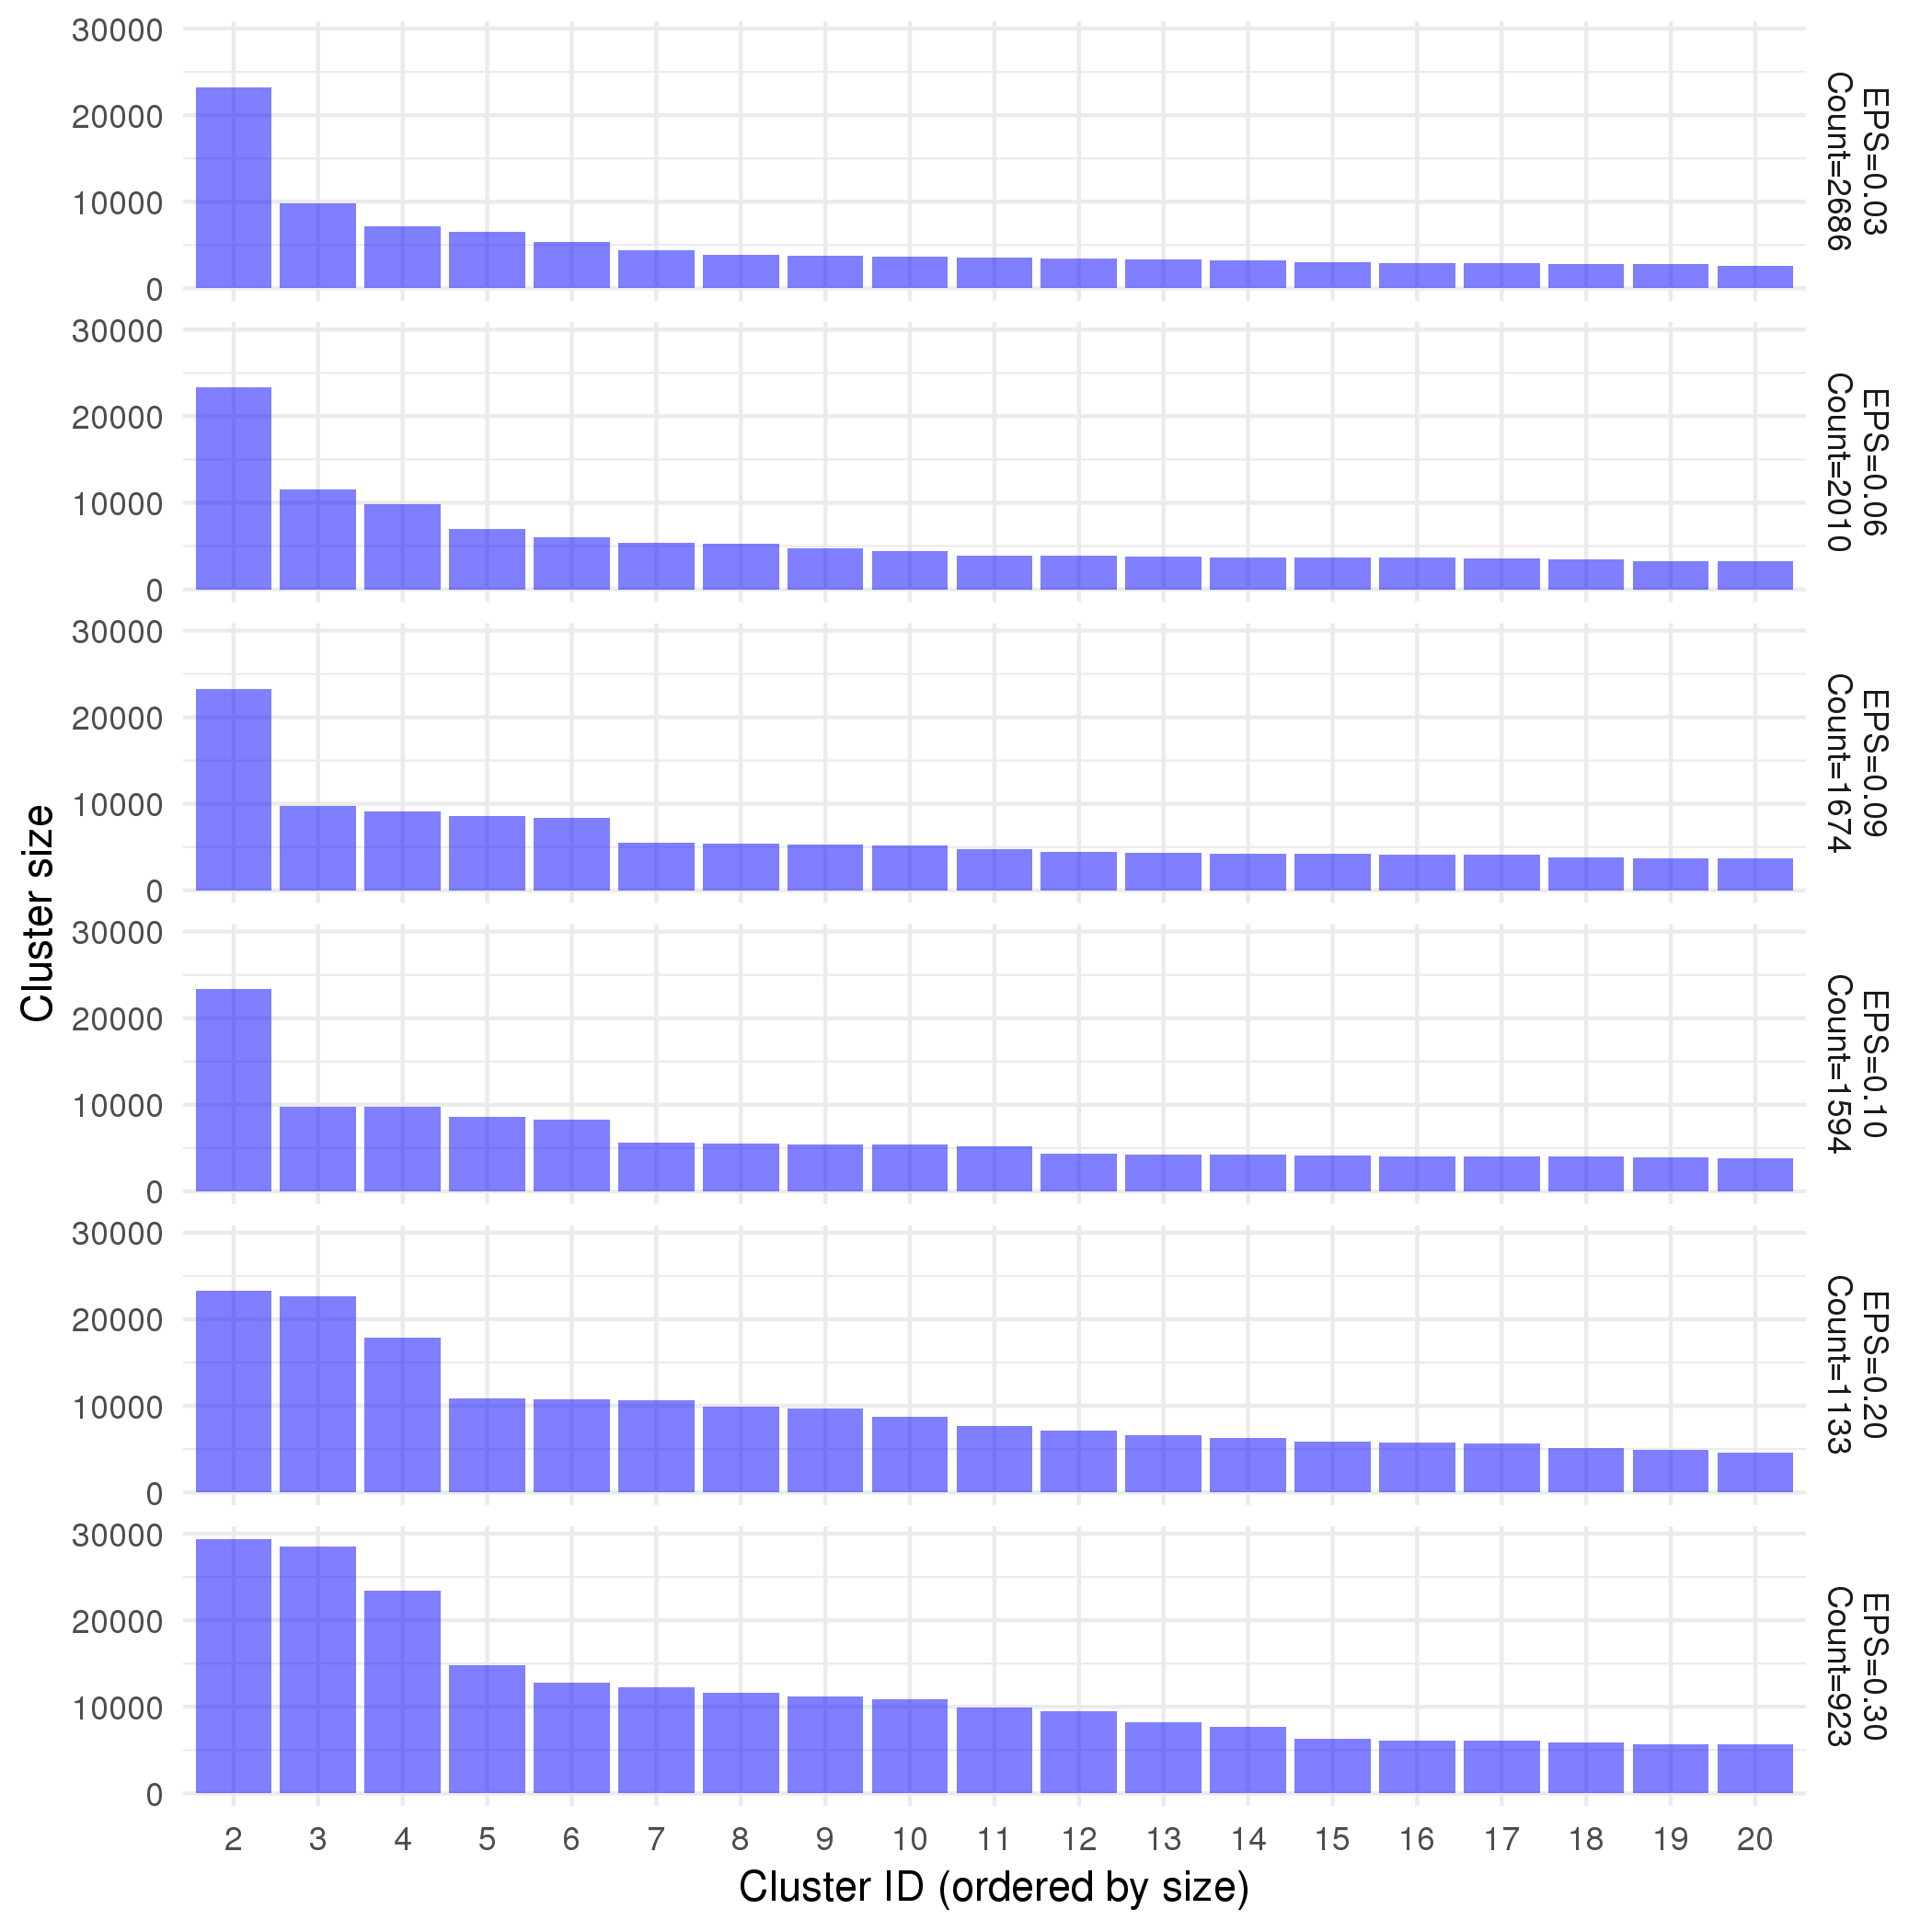
\includegraphics[width=\textwidth]{./media/image12.png}
	\caption{Job-IO-Metric}
	\label{fig:datasets_clustering_results:io_metric}
 \end{subfigure}
 \caption{The Top 20 largest clusters.}
 \label{fig:datasets_clustering_results}
\end{figure}

\subsubsection{Clustering of the Job-IO-Metric and Job-IO-Duration datasets}
As already mentioned in the related work section, the Job-IO-Metric dataset has 3 features, Job-I/O-Balance, Job-I/O-Utilization, and Job-I/O-Problem-Time.
After the data pre-processing, we obtain a set of 3-dimensional data points with a domain between 0 and 1.
According to the formula, the EPS\_MAX is 1.44.
We conducted several experiments with different EPS values between 0 and EPS\_MAX and visualized the results in \Cref{fig:datasets_clustering_results:io_metric} on the right side.
It shows the cluster sizes of Top 20 largest clusters and the total number of clusters.

The\ Job-IO-Duration dataset contains the fraction of runtime jobs spent doing I/O.
 The 27 columns are named according to the following scheme: metric\_category, e.g, bytes\_read\_0 or md\_file\_delete\_4.
The first part is the one of the nine metric names and the second part is the category number (LowIO=0, HighIO=1 and CriticalIO=4).
These columns are used for machine learning as input features.
There is a constraint for each metric (metric\_0 + metric\_1 + metric\_4 = 1), that makes 9 features redundant, because they can be computed from the other features, so that we have to deal with 18 features only, and EPS\_MAX is 1.17.
We visualized the results in \Cref{fig:datasets_clustering_results:io_duration} on the left side.

A look inside clusters reveals chaotic clustering results.
For both datasets and for all EPS values we could find many coding sequences in a cluster that don't belong in the same cluster.
For example a cluster can contain the following sequences.

\begin{lstlisting}
[1], [0:0:14:0], [4:0], [0:0:4:0], [272:272:272] 
\end{lstlisting}

We look at least in the Top 10 largest clusters and find the same picture for all of the.
Even with low EPS values the algorithms produce many polluted clusters, i.e, with samples from other clusters.
Like in the example above, we could find any logic behind the results.
Probably, these particular datasets do not represent the specifics of parallel jobs not well enough for proper clustering, but even with a good feature set that works on our test system, there is no guarantee that the approach will be portable to other systems.

\subsection{Evaluation of custom clustering algorithms}
This section contains data statistics, clustering progress, and clustering results of codings with the five customized algorithms (BIN\_ALL, BIN\_AGGZEROS, HEX\_LEV, HEX\_NATIVE, PM\_QUANT).
Due to lack of tools, we determine cluster quality on a small scale.

\subsubsection{Test setup}
For the performance tests we allocate a compute node on Mistral supercomputer.
It is equipped with 2x Intel(R) Xeon(R) CPU E5-2680 v3 @ 2.50GHz, 64GB DDR4 RAM.
The clustering algorithms are implemented in Rust and run on a single core.

\subsubsection{SIM value exploration}
In the introduced algorithms, the SIM value controls the cluster formation.
In the course of evaluation, we will show that low SIM values produce a small amount, but polluted clusters, and a high SIM value produces a large amount, but clean clusters.
We suppose the optimal value is somewhere in between.

First\ of all, we observe the clustering progress by recording  the number of created clusters after each 10.000 jobs.
The clustering progress is visualized in \Cref{fig:clustering_progress}.
The gradient of the curve shows the generalization capabilities of each algorithm for different SIM values.

When looking for the optimal SIM, we created the following criteria.
Firstly, we need to select a SIM value, just before the increase of the SIM value doesn't make significant improvements.
PM and BIN algorithms work best for SIM values between 0.7 and 0.9, and for HEX the SIM value between 0.95 and 0.99.
We can also observe flattening curves with increasing numbers of jobs, which indicates that more jobs are placed in clusters and less clusters are created.

\begin{figure}
  \centering
   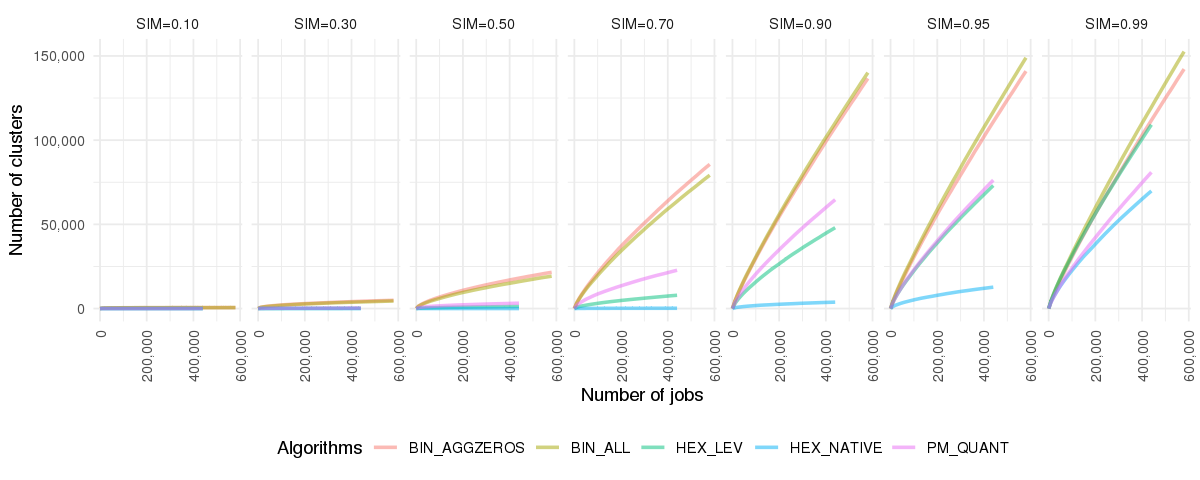
\includegraphics[width=4.61in,height=1.85in]{./media/image15.png}
   \caption{Clustering progress.}
   \label{fig:clustering_progress}
\end{figure}

Although an optimal SIM value is depending on use case and dataset, a parameter exploration may provide important hints to find a good value and achieve optimal cluster qualities.
\Cref{fig:clustering_progress} visualizes the cluster creation for different SIM values.
The red line approximates the overall number of clusters, the green line shows how many contain at least two jobs and the blue line shows how many of them contain at least 10 jobs.

Coding with 100$\%$  similarity are of the same job type, i.e, they have exactly the same length and I/O behavior.
In \Cref{fig:clustering_progress} the threshold is visualized by the grey line.


Apparently, for each algorithm (except HEX) there is some SIM value, when the clustering algorithms start working contra-productive, i.e., the number of clusters with more than two jobs is decreasing.
This happens, because more clusters are splitted in individual jobs than created.
That is something we usually want to prevent, because the algorithms stop finding similar jobs, but focus on refining clusters.

\Cref{fig:alg_runtimes} shows the clustering runtimes of clustering a total number of jobs with increments of 10,000 jobs, i.e., each point represents the runtime for a given number of total jobs.
The clustering time depends heavily on the number of created clusters (see \Cref{fig:clustering_progress}).
The reason is that the algorithm tries to put each job in existing clusters first.
It iterates over them, and only if it is not able to find a suitable cluster, it creates a new one.
The more clusters exist, the longer is the processing time.
Since, for low SIM values there are low number of clusters, the clustering is much faster.
PM\_QUANT has exceptionally high runtimes due to quadratic runtimes of phase matching.
In one case the runtimes clustering of 10,000 jobs took up to 4.3 hours (the outliers are not shown in the picture).
We suppose, this lies on the quadratic runtimes of the phase matching procedure.
We didn't spend time to optimize the algorithm further.

\begin{figure}
  \centering
  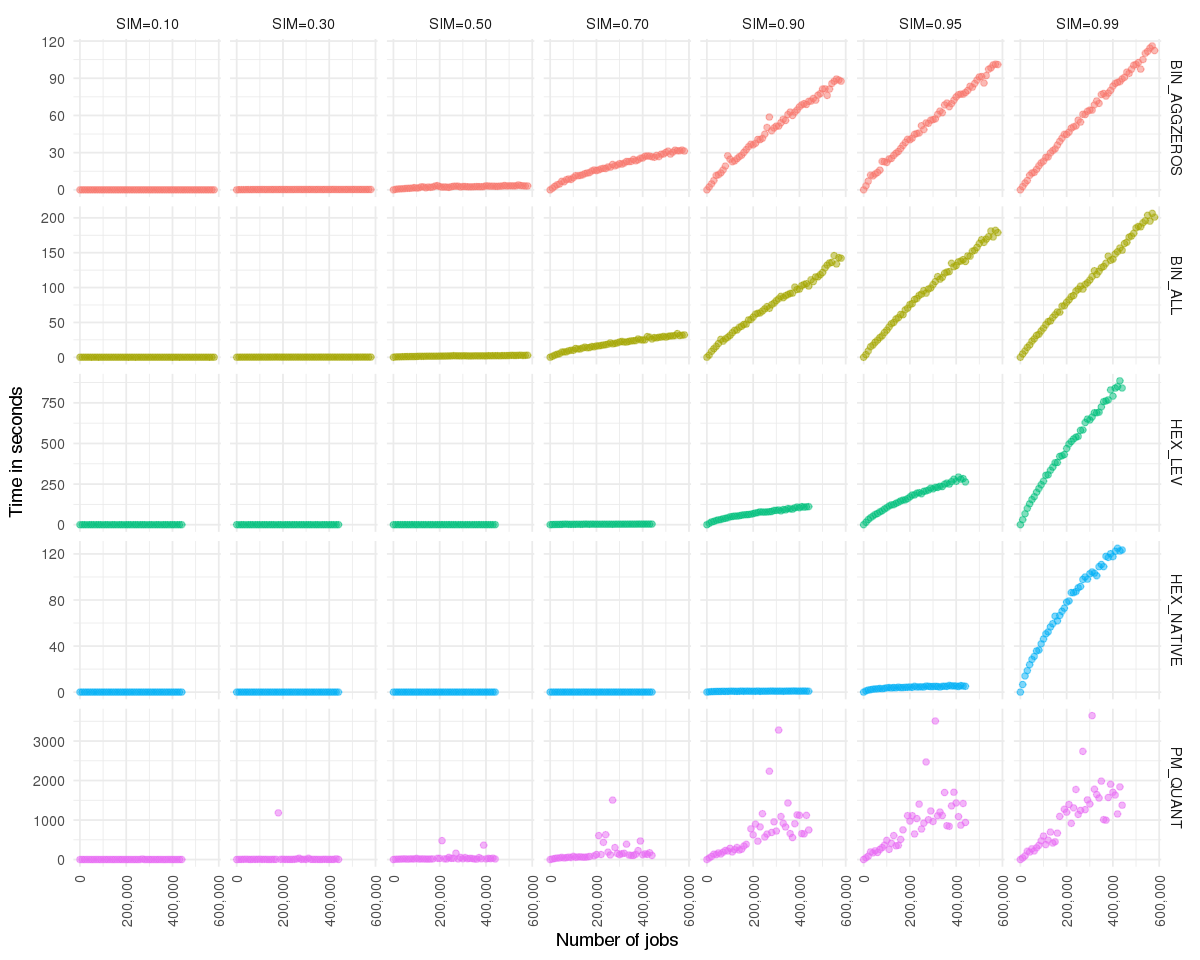
\includegraphics[width=4.61in,height=3.68in]{./media/image18.png}
  \caption{Runtime for executing the clustering.}
  \label{fig:alg_runtimes}
\end{figure}

\begin{figure}
  \centering
  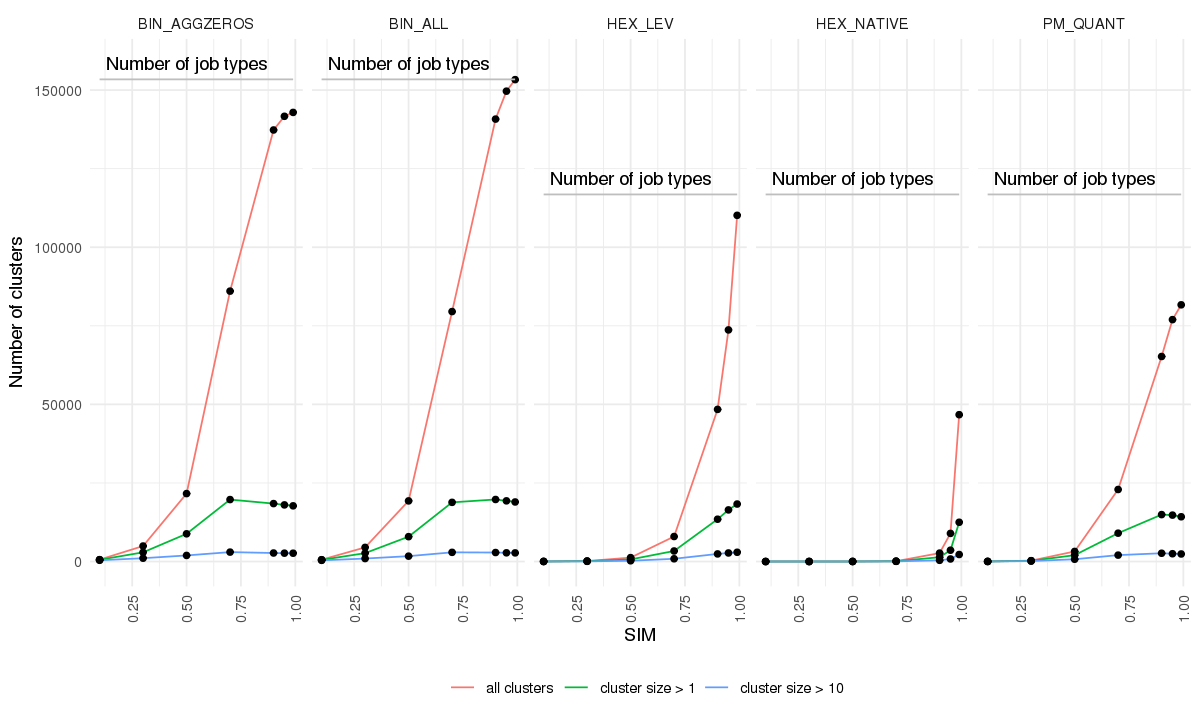
\includegraphics[width=4.61in,height=2.76in]{./media/image19.png}
  \caption{Similarity value exploration.}
  \label{fig:sim_eploration}
\end{figure}

\begin{figure}
  \centering
  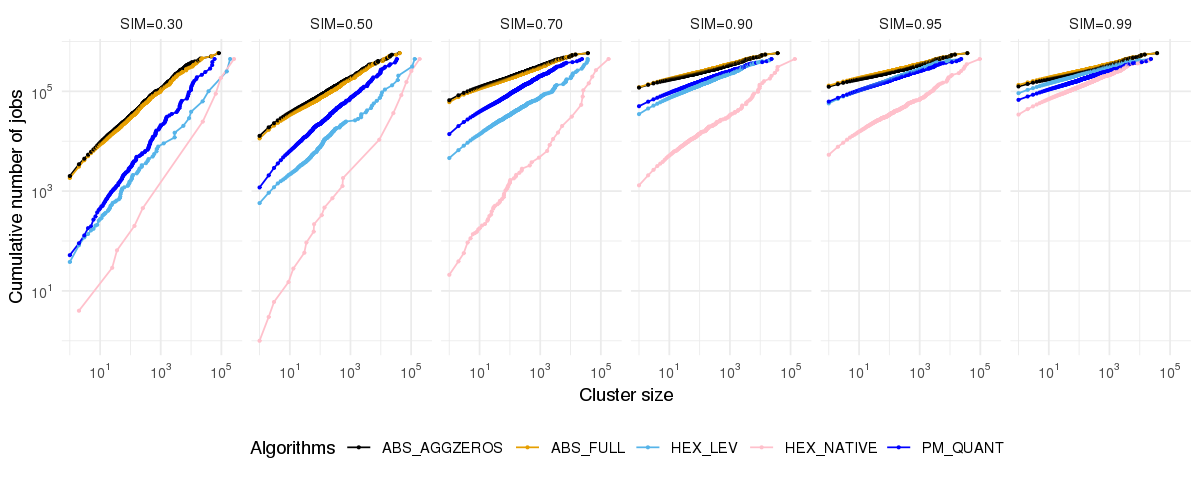
\includegraphics[width=4.61in,height=1.85in]{./media/image22.png}
  \caption{Cumulative number of jobs with different sizes.}
  \label{fig:cum_num_job_sizes}
\end{figure}

Another quality indicator is the number of small clusters.
\Cref{fig:cum_num_job_sizes} the final clustering result.
Obviously, the ABS algorithms tend to create many small clusters.
In these terms, PM behaves much better and HEX best.
A quite interesting observation is that after scaling both axes with log10 function, we can observe a kind linearity for all algorithms.

The\ previous investigations have no meaning, if cluster quality is bad.
To give you an  impression of cluster qualities for different SIM values, we define the relevance by the equation below and we visualize the Top 10 relevant clusters in
\Cref{fig:top10_relevant_jobs}.
The colors indicate the mean similarity of jobs to the cluster centroid.
The number above the bar denotes the mean job length of the cluster.

\begin{figure}
  \centering
  
\includegraphics[width=2.5in,height=0.12in]{./media/image16.png}
  \caption{Equation}
  \label{fig:equation}
\end{figure}

%~\href{https://www.codecogs.com/eqnedit.php?latex=%5Ctext%7BRelevance%7D%3D%5Ctext%7BClusterSize%7D%5Ccdot%5Ctext%7BMeanJobLength%7D#0}{}

The idea behind the relevance definition is the following: the larger the cluster and the longer the jobs, the more potential load these jobs can produce.
Therefore it is worth investigating these clusters first.
In principle, the figure confirms that SIM values larger than optimum provide not much improvement, but nevertheless, it does not mean that the cluster quality is acceptable.
After investigation of some clusters we noticed SIM value independent characteristics.
To explain them, it is sufficient to look in one cluster of each algorithm, as we do in the next sections.

\begin{figure}
  \centering
   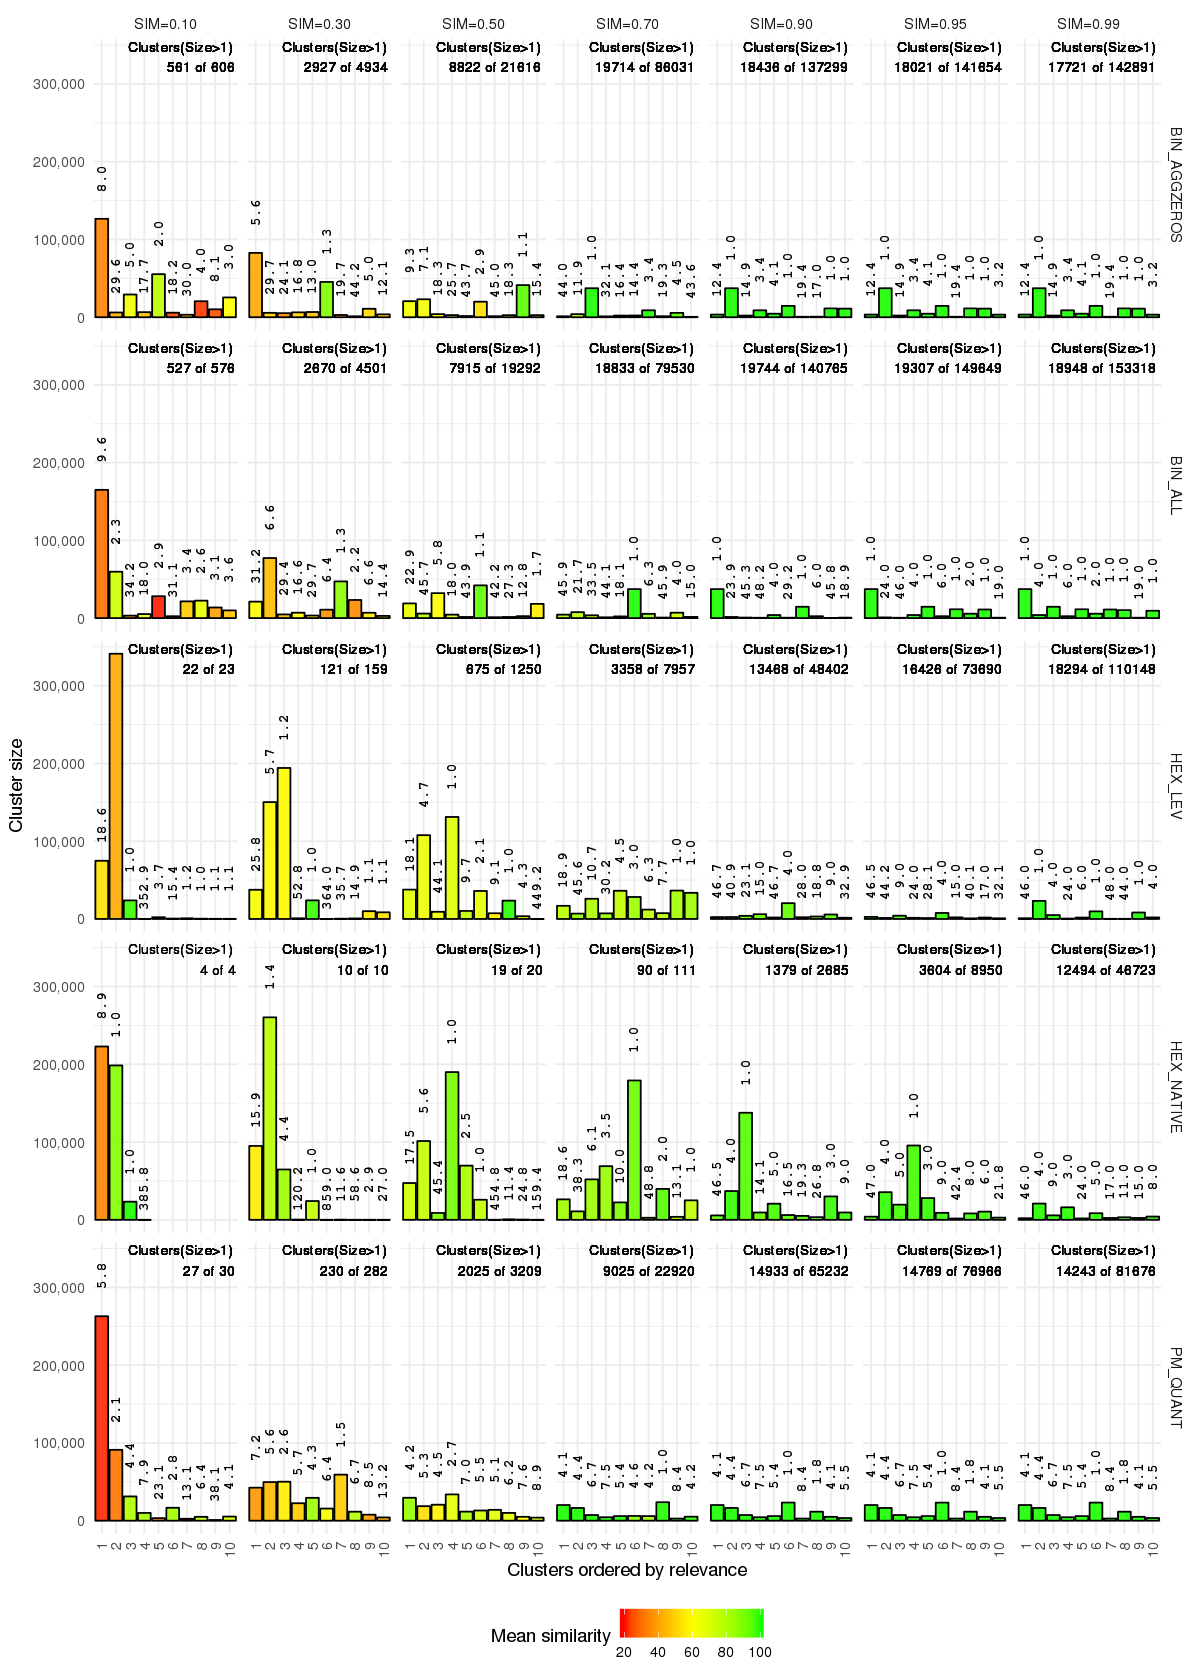
\includegraphics[width=4.61in,height=6.44in]{./media/image11.png}
   \caption{Top 10 relevant jobs ordered by relevance.}
   \label{fig:top10_relevant_jobs}
\end{figure}

\subsubsection{Cluster presentation format}

The next sections we have the following format, a description of any particular observations if necessary, followed by a table containing the most important statistics, and by the codings for job, centroid and and the Top 5 job types.
At the end we include an illustration which describe the length distribution of the cluster.


\subsubsection{Algorithm characteristics}
\paragraph{BIN\_ALL}
%\Cref{tab:bin:largest_clusters}, \textcolor[HTML]{1155CC}{\uline{Table 8}}, \textcolor[HTML]{1155CC}{\uline{Table 9}}, and \textcolor[HTML]{1155CC}{\uline{Figure 10}}.
Information related to the cluster is in \Cref{tab:bin:largest_clusters}, \Cref{tab:bin_all:stats}, \Cref{tab:bin_all:top_jobs}, and \Cref{fig:bin_all:length}.

One of the first observations we did for BIN family algorithms is that the six largest clusters contain the shortest jobs (one segment long).
They are listed in \Cref{tab:bin:largest_clusters}.
All jobs in each cluster have exactly the same codings.
The reason that both algorithms create the same clusters, is that the zero aggregation has no effect on formation of these clusters, because the jobs are too short (the minimum job length required for effective zero aggregation is at least three segments) and that the dataset contains a vast amount of such jobs.
The largest cluster is even representative in Top10 relevant jobs in ref\_top\_ten.

%\begin{table}[h]
\begingroup
  \centering
  \begin{tabular}{ll}
    Coding sequence & Cluster size \\
    \hline
    $[511]$ & 37,272 \\ 
    $[32]$  & 14,536 \\ 
    $[272]$ & 11,338 \\ 
    $[160]$ & 11,014 \\ 
    $[128]$ & 10,228 \\ 
    $[8]$   & 9,446  \\ 
  \end{tabular}
	\captionof{table}{Top 6 largest clusters created by BIN algorithms with SIM = 0.7.}
  \label{tab:bin:largest_clusters}
\endgroup
%\end{table}

Most jobs in the cluster are shorter than 49 segments, because the main Mistral partitions can allocate jobs for at most 8 hours, and that is the majority of jobs.
The other jobs must be special allocations.
Since each segment is 10 min long, the runtime of jobs with 49 segments is about 8.16 hours.
The other jobs must be special allocations or jobs from other partitions.

The following observations are characteristic for this algorithm:
\begin{enumerate}
 \item Job types can significantly differ from centroid and from each other.
 \item Lengths of job types in a cluster are relatively close to the centroid.
\end{enumerate}

%\begin{table}[h]
\begingroup
  \centering
  \begin{tabular}{lr}
    SIM & 0.7 \\
    Number of jobs & 7615 \\
    Number of job types & 3306 \\
  \end{tabular}
	\captionof{table}{Cluster statistics.}
  \label{tab:bin_all:stats}
\endgroup
%\end{table}

%\begin{table}[h]
\begingroup
  \centering
  \begin{tiny}
    \begin{tabular}{@{ }l@{ }|@{ }r@{ }}
			\rowcolor{tabhcolor}\rowstyle{\bfseries}
      Binary coding                                                                                    &  Type     \\ 
      \hline
      0:0:0:0:0:0:294:0:0:0:0:32:0:0:0:0:0:0:0:0:0:0:0:32:0:0:0:0:0:0:0:0:0:0:0:32:0:0:0:0:0:0:0:0:0:0 &  centroid \\ 
      \multicolumn{2}{l}{}                                                                             \\ 
			\rowcolor{tabhcolor}\rowstyle{\bfseries}
      Binary coding                                                                                    &  Count    \\ 
      \hline
      0:0:0:0:0:0:359:96:0:0:0:0:0:0:0:0:0:0:0:0:0:0:0:0:0:0:0:0:0:0:0:0:0:0:0:0:0:0:0:0:0:0:0:0:0:0   &  95       \\ 
      0:0:0:0:0:0:295:0:0:0:0:0:0:0:0:0:0:0:0:0:0:0:0:0:0:0:0:0:0:0:0:0:0:0:0:0:0:0:0:0:0:0:0:0:0:0    &  62       \\ 
      0:0:0:0:0:0:0:0:0:0:0:0:4:0:0:0:0:0:0:0:0:0:0:0:0:0:0:0:0:0:0:0:0:0:0:0:0:0:0:0:0:0:0:0:0:0:0:0  &  47       \\ 
      0:0:0:0:0:0:359:0:0:0:0:0:0:0:0:0:0:0:0:0:0:0:0:0:0:0:0:0:0:0:0:0:0:0:0:0:0:0:0:0:0:0:0:0:0:0    &  44       \\ 
      0:0:0:0:0:6:6:0:0:0:0:0:0:0:0:0:0:0:0:0:0:0:0:0:0:0:0:0:0:0:0:0:0:0:0:0:0:0:0:0:0:0:0:0:0:0:0:0  &  40       \\ 
    \end{tabular}
  \end{tiny}
	\captionof{table}{Centroid and Top 5 job types.}
  \label{tab:bin_all:top_jobs}
\endgroup
%\end{table}

%\begin{figure}[h]
\begingroup
  \centering
  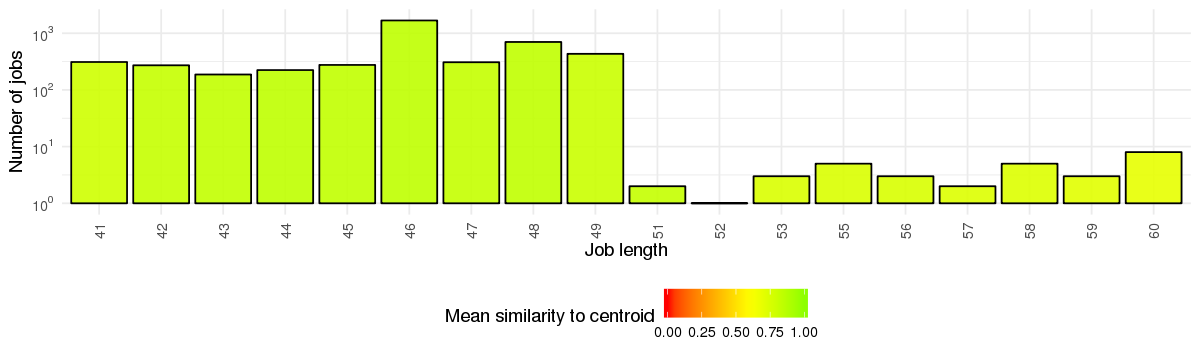
\includegraphics[width=4.61in,height=1.39in]{./media/image20.png}
	\captionof{table}{Length distribution in the cluster.}
  \label{fig:bin_all:length}
\endgroup
%\end{figure}


\paragraph{BIN\_AGGZEROS}
Information related to the cluster is in \Cref{tab:bin_aggzeros:stats}, \Cref{tab:bin_aggzeros:top_jobs}, and in \Cref{fig:bin_aggzeros:length}.

The following is characteristic for this algorithm:

\begin{enumerate}
 \item Job types can significantly differ from centroid and from each other.
 \item Lengths of job types in a cluster are relatively far from the centroid and compared to BIN\_ALL.
 \item I/O intensive clusters appear to be cleaner than BIN\_ALL.
\end{enumerate}

%\begin{table}[h]
\begingroup
  \begin{tabular}{ll}
    \centering
    SIM &  0.7 \\
    Number of jobs & 1295 \\
    Number of job types & 336 \\
  \end{tabular}
	\captionof{table}{Cluster statistics.}
  \label{tab:bin_aggzeros:stats}
\endgroup
%\end{table}

%\begin{table}[h]
\begingroup
  \centering
  \begin{tiny}
    \begin{tabular}{@{ }l@{ }|@{ }r@{ }}
			\rowcolor{tabhcolor}\rowstyle{\bfseries}
      Binary coding                                                                          &  Type     \\ 
      \hline
      272:272:272:272:272:278:286:272:272:272:272:272:272:272:272:272:272:272:272            &  centroid \\ 
      \multicolumn{2}{l}{}                                                                   \\ 
      \hline
			\rowcolor{tabhcolor}\rowstyle{\bfseries}
      Binary coding                                                                          &  Count    \\ 
      272:272:272:272:272:278:286:272:272:272:272:272:272:272:272:272:272:272:272            &  528      \\ 
      272:272:272:272:272:406:286:272:272:272:272:272:272:272:272:272                        &  96       \\ 
      272:272:272:272:272:279:31:272:272:272:272:272:272:272:272:272:272:272:272:272:272:272 &  53       \\ 
      272:272:272:272:272:272:272:272:272:272:272:279:319:272:272:272:272:272:272:272:272    &  52       \\ 
      272:272:272:272:272:279:319:272:272:272:272:272:272:272:272:272:272:272:272:272:272    &  50       \\ 
    \end{tabular}
  \end{tiny}
	\captionof{table}{Centroid and Top 5 job types}
  \label{tab:bin_aggzeros:top_jobs}
\endgroup
%\end{table}

%\begin{figure}[h]
\begingroup
  \centering
  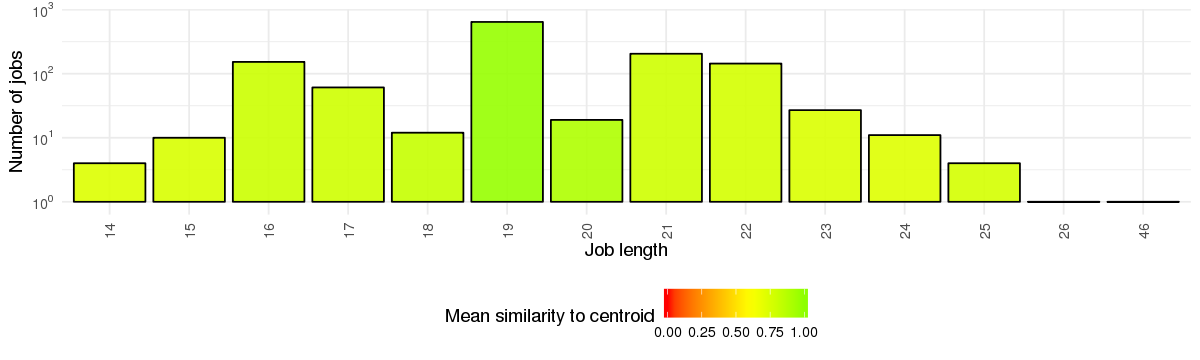
\includegraphics[width=4.61in,height=1.38in]{./media/image13.png}
	\captionof{figure}{Job length distribution in the cluster.}
  \label{fig:bin_aggzeros:length}
\endgroup
%\end{figure}


\paragraph{HEX\_LEV}
Information related to the cluster is in \Cref{tab:hex_lev:stats}, \Cref{tab:hex_lev:top_jobs}, and in \Cref{fig:hex_lev:length}.

HEX\_LEV reacts slowly to the increasing SIM value, due to the longer hexadecimal codings, compared to binary codings.
Therefore, we chose a SIM value higher than for BIN algorithms.
But even with a high SIM value, we can observe that some jobs have a different I/O behavior than the centroid and the rest of the jobs.
The reason is that Levenshtein distance is not performance aware, i.e., the distance between value 1 and 2 is the same as for 1 and 8.
There is no such a job in the example below, but we can observe this in other clusters.

Cluster characteristics:

\begin{enumerate}
 \item Similar job lengths
 \item Mostly clean clusters, but can contain outlier jobs
\end{enumerate}

%\begin{table}[h]
\begingroup
	\centering
	\begin{tabular}{ll}
		SIM & 0.9 \\
		Number of jobs & 5769 \\
		Number of job types & 2473 \\
	\end{tabular}
	\captionof{table}{Cluster statistics.}
	\label{tab:hex_lev:stats}
\endgroup
%\end{table}


%\begin{table}[h]
\begingroup
  \centering
  \begin{tiny}
    \begin{tabular}{@{ }l@{ }@{ }l@{ }@{ }l@{ }@{ }l@{ }|@{ }r@{ }}
			\rowcolor{tabhcolor}
      \multicolumn{4}{@{ }l|@{ }}{\rowstyle{\bfseries}Hexadecimal coding} & \\
			\rowcolor{tabhcolor}\rowstyle{\bfseries}
      md\_file\_create  & md\_file\_delete  & md\_mod           & read\_calls       & Type     \\ 
      \hline
      0:...:0           & 0:0:0:1:0:0:0:0:0 & 0:...:0           & 0:...:0           & centroid \\ 
      \multicolumn{5}{l}{}\\
			\rowcolor{tabhcolor}\rowstyle{\bfseries}
      md\_file\_create  & md\_file\_delete  & md\_mod           & read\_calls       & Count    \\ 
      \hline
      0:...:0           & 0:0:0:0:0:0:1:0:0 & 0:...:0           & 0:...:0           & 606      \\ 
      0:...:0           & 0:0:0:0:0:0:0:0:1 & 0:...:0           & 0:...:0           & 562      \\ 
      0:...:0           & 0:...:0           & 0:...:0           & 0:0:0:0:0:0:1:0:0 & 429      \\ 
      0:...:0           & 0:0:0:1:0:0:0:0:0 & 0:...:0           & 0:...:0           & 185      \\ 
      0:0:0:0:0:0:1:1:1 & 0:...:0           & 0:0:0:0:0:0:1:0:0 & 0:...:0           & 75       \\ 
    \end{tabular}
  \end{tiny}
	\captionof{table}{Centroid and Top 5 job types}
  \label{tab:hex_lev:top_jobs}
\endgroup
%\end{table}


%\begin{figure}[h]
\begingroup
  \centering
  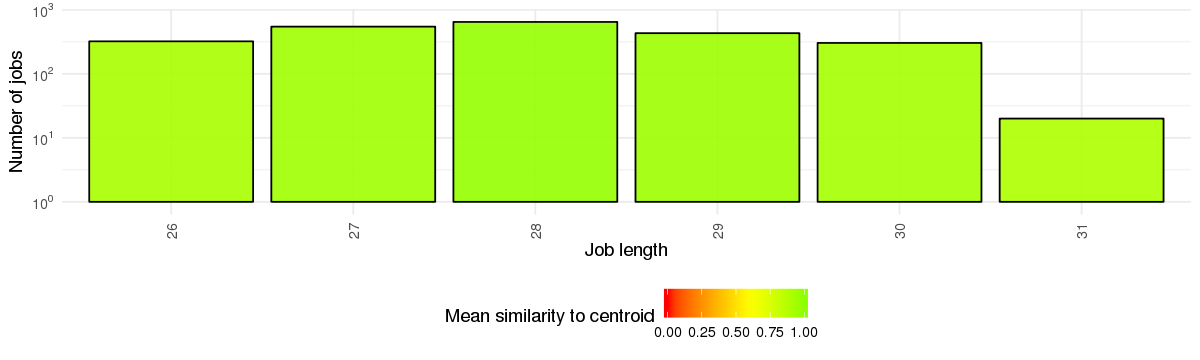
\includegraphics[width=4.61in,height=1.39in]{./media/image5.png}
	\captionof{figure}{Length distribution in the cluster.}
  \label{fig:hex_lev:length}
\endgroup
%\end{figure}


\paragraph{HEX\_NATIVE}
Information related to the cluster is in \Cref{tab:hex_native:stats}, \Cref{tab:hex_native:top_jobs}, and in \Cref{fig:hex_native:length}.

The SIM value exploration shows, that this algorithm works best with high SIM values.
Clustering with SIM=0.99 results in clusters that have equal job lengths.
(For SIM=0.99 the centroid must be longer than 100 segments to attract jobs with other lengths.) 

Cluster characteristics:

\begin{enumerate}
 \item Similar job lengths
 \item Jobs are relatively close to the centroid
 \item Low number of outliers
\end{enumerate}

%\begin{table}[h]
\begingroup
  \centering
  \begin{tabular}{ll}
    SIM & 0.99 \\
    Number of jobs & 20908 \\
    Number of job types & 11997 \\
  \end{tabular}
	\captionof{table}{Cluster statistics.}
  \label{tab:hex_native:stats}
\endgroup
%\end{table}


%\begin{table}[h]
\begingroup
  \centering
  \begin{tiny}
    \begin{tabular}{@{ }l@{ }@{ }l@{ }@{ }l@{ }|@{ }r@{ }}
			\rowcolor{tabhcolor}
      \multicolumn{3}{@{ }l|@{ }}{\rowstyle{\bfseries}Hexadecimal coding} &            \\ 
			\rowcolor{tabhcolor}\rowstyle{\bfseries}
      md\_file\_delete     &  md\_mod   & md\_other & Type     \\ 
      \hline
      0:\dots:0            &  0:0:1:0   & 0:0:1:0   & centroid \\ 
      \multicolumn{4}{l}{} \\ 
			\rowcolor{tabhcolor}\rowstyle{\bfseries}
      md\_file\_delete     &  md\_mod   & md\_other & Count    \\ 
      \hline
      0:\dots:0            &  0:\dots:0 & 0:0:1:0   & 5,010    \\ 
      0:\dots:0            &  0:\dots:0 & 0:0:2:0   & 1,963    \\ 
      0:0:1:0              &  0:\dots:0 & 0:\dots:0 & 1,099    \\ 
      0:\dots:0            &  0:\dots:0 & 0:1:0:0   & 911      \\ 
      0:0:1:0              &  0:0:1:0   & 0:\dots:0 & 676      \\ 
    \end{tabular}
  \end{tiny}
	\captionof{table}{Centroid and Top 5 job types.}
  \label{tab:hex_native:top_jobs}
\endgroup
%\end{table}


%\begin{figure}[h]
\begingroup
  \centering
  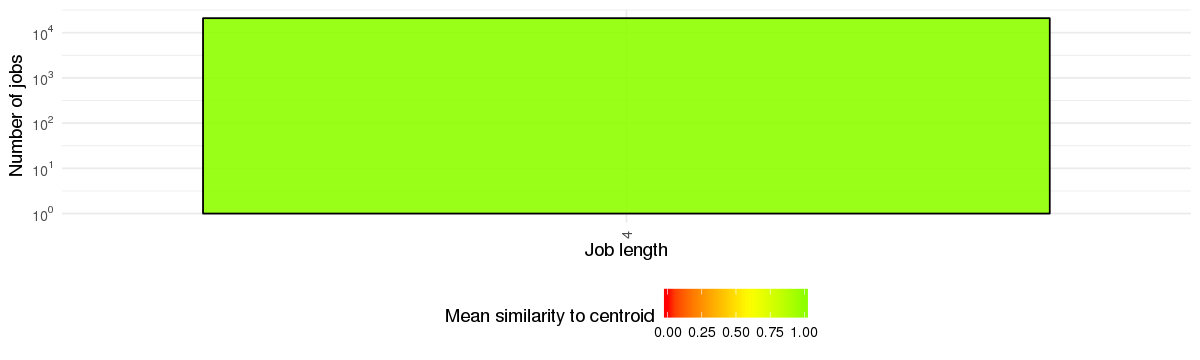
\includegraphics[width=4.61in,height=1.39in]{./media/image8.png}
	\captionof{figure}{Length distribution in the cluster.}
  \label{fig:hex_native:length}
\endgroup
%\end{figure}





\paragraph{PM\_QUANT}
Information\ related to the cluster is in \Cref{fig:pm_quant:stats}, \Cref{fig:pm_quant:top_jobs}, and in \Cref{fig:pm_quant:length}.

The first thing to mention are the high generalization capabilities of the algorithm, i.e., that many jobs are mapped to a relatively low number of types.
The next typical property is shown in \Cref{fig:pm_quant:length}, where we can see that almost the full range of job lengths is represented in the cluster.
This happens, because the PM ignores zero segments completely.
We saw that already in BIN\_AGGZEROS, where a similar effect was caused by the aggregation of zero segments.
For example, for PM, the job types in \Cref{fig:pm_quant:top_jobs} in the row one and two are 100$\%$  similar.
Remarkable is also the cleanliness of the clusters.
The centroid and the jobs contain quite similar I/O patterns.

Cluster characteristics:

\begin{enumerate}
 \item Low number of job types
 \item Relatively large number of job lengths
 \item I/O pattern 
\end{enumerate}

%\begin{table}[h]
\begingroup
  \centering
  \begin{tabular}{ll}
    SIM & 0.7 \\
    Number of jobs & 5175 \\
    Number of job types & 154 \\
  \end{tabular}
	\captionof{table}{Cluster statistics.}
  \label{fig:pm_quant:stats}
\endgroup
%\end{table}

%\begin{table}[h]
\begingroup
  \centering
  \begin{tiny}
    \begin{tabular}{@{ }l@{ }@{ }l@{ }|@{ }r@{ }}
			\rowcolor{tabhcolor}
			\multicolumn{2}{@{ }l|@{ }}{\rowstyle{\bfseries}Hexadecimal coding} &              \\ 
			\rowcolor{tabhcolor}\rowstyle{\bfseries}
      md\_file\_delete     &  md\_mod     & Type     \\ 
      \hline
      4:0:0:0:0:0          &  4:0:0:0:0:0 & centroid \\ 
      \multicolumn{3}{l}{} \\ 
			\rowcolor{tabhcolor}\rowstyle{\bfseries}
      md\_file\_delete     &  md\_mod     & Count    \\ 
      \hline
      4                    &  4           & 2329     \\ 
      4:0:0:0:0:0          &  4:0:0:0:0:0 & 1773     \\ 
      4:0                  &  4:0         & 224      \\ 
      2                    &  4           & 65       \\ 
      0:4                  &  0:4         & 57       \\ 
    \end{tabular}
  \end{tiny}
	\captionof{table}{Centroid and Top 5 job types.}
  \label{fig:pm_quant:top_jobs}
\endgroup
%\end{table}

%\begin{figure}[h]
\begingroup
  \centering
  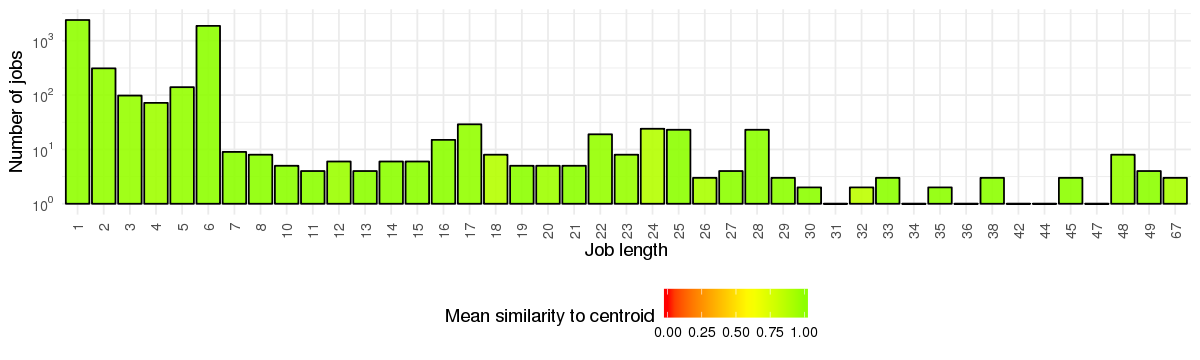
\includegraphics[width=4.61in,height=1.39in]{./media/image21.png}
	\captionof{figure}{Length distribution in the cluster.}
  \label{fig:pm_quant:length}
\endgroup
%\end{figure}

\subsection{Use case: I/O intensive job}
The demonstration in this section shows how this approach can be used to identify a cluster of I/O-intensive jobs similar to an existing job.

\begin{figure}[h]
  \centering
  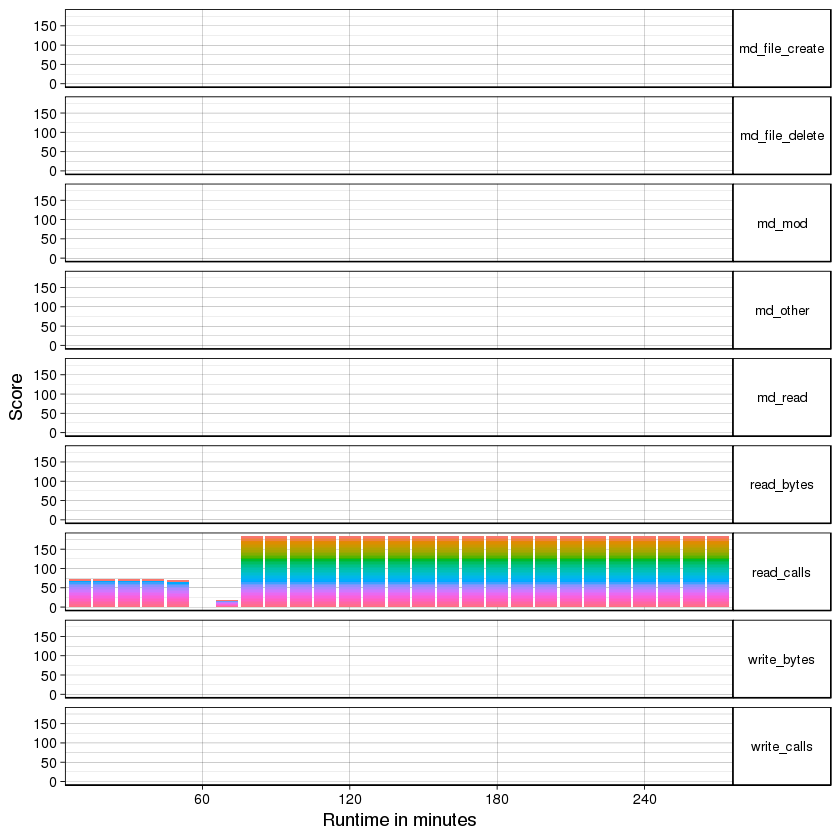
\includegraphics[width=2.84in,height=2.85in]{./media/image1.png}
  \caption{One high I/O intensity job running on 46 nodes. Score is the sum of all nodes stacked by the node. A color represents one of the nodes.}
  \label{fig:use_case}
\end{figure}

Firstly,\ we find a job that we like to identify similar jobs.
To do that, we rank jobs by using the equation below and pick a job from the top of the sorted list.
The selected job is visualized in \Cref{fig:use_case}.
We can see that this job reads data over the whole runtime.
At beginning, only a subset of the nodes is reading most of the data, later more nodes participate in the reading The amount of transmitted data is not large, but the amount of read calls is exceptionally high and may potentially degrade the file system performance.
Now we investigate the cluster that contains this job for the different algorithms.

\paragraph{BIN\_ALL}
Information related to the cluster is in \Cref{tab:use_case:bin_all:stats}, \Cref{tab:use_case:bin_all:top_jobs}, and in \Cref{fig:use_case:bin_all:length}.

%\begin{table}[h]
\begingroup
  \centering
  \begin{tabular}{ll}
    SIM & 0.7 \\
    Number of jobs & 27 \\
    Number of job types & 17 \\
  \end{tabular}
	\captionof{table}{Cluster statistics.}
  \label{tab:use_case:bin_all:stats}
\endgroup
%\end{table}

%\begin{table}[h]
\begingroup
  \centering
  \begin{tiny}
    \begin{tabular}{@{ }l@{ }|@{ }r@{ }}
			\rowcolor{tabhcolor}\rowstyle{\bfseries}
      Binary coding                                                                                          &  Type     \\ 
      \hline
      192:192:192:192:192:192:196:192:192:192:192:192:192:192:192:192:192:192:192:192:192:192:64:64:64:64:64 &  job      \\ 
      192:192:192:192:192:192:192:192:192:192:192:454:230:192:192:192:192:192:192:192:192:192:192:192        &  centroid \\ 
      \multicolumn{2}{l}{}                                                                                   \\ 
			\rowcolor{tabhcolor}\rowstyle{\bfseries}
      Binary coding                                                                                          &  Count    \\ 
      \hline
      192:192:192:192:192:454:198:192:192:192:192:192:192:192:192:192:192:192:192:192:192:192:192:192        &  5        \\ 
      192:192:192:192:192:192:192:192:192:192:192:454:230:192:192:192:192:192:192:192:192:192:192:192        &  3        \\ 
      192:192:192:192:192:454:230:192:192:192:192:192:192:192:192:192:192:192:192:192:192:192:192:192        &  3        \\ 
      192:192:192:192:192:192:192:192:192:192:192:454:230:192:192:192:192:192:192:192:192:192:192            &  2        \\ 
      228:192:192:192:192:192:192:192:192:192:192:192:192:192:192:192:192:192                                &  2        \\ 
    \end{tabular}
  \end{tiny}
	\captionof{table}{Job, centroid and Top 5 job types.}
  \label{tab:use_case:bin_all:top_jobs}
\endgroup
%\end{table}

%\begin{figure}[h]
\begingroup
  \centering
  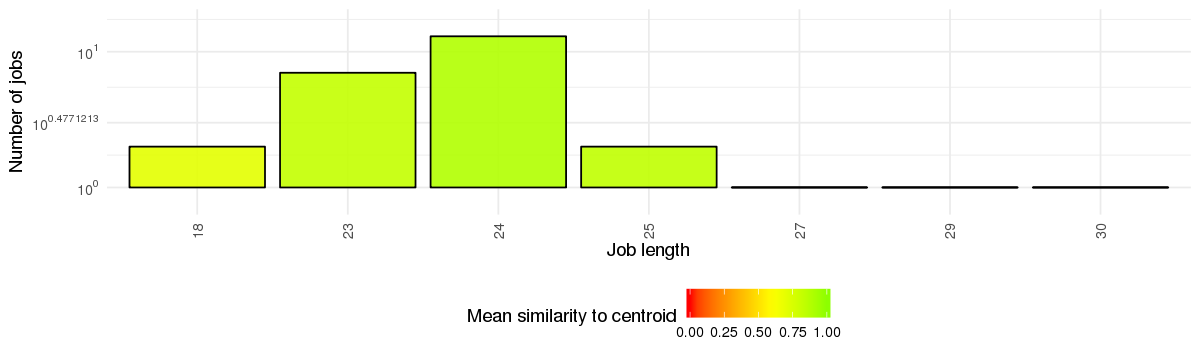
\includegraphics[width=4.61in,height=1.39in]{./media/image9.png}
	\captionof{figure}{Length distribution in the cluster.}
  \label{fig:use_case:bin_all:length}
\endgroup
%\end{figure}


\paragraph{BIN\_AGGZEROS}
Information related to the cluster is in \Cref{tab:use_case:bin_aggzeros:stats}, \Cref{tab:use_case:bin_aggzeros:top_jobs}, and in \Cref{fig:use_case:bin_aggzeros:length}.

%\begin{table}[h]
\begingroup
  \centering
  \begin{tabular}{ll}
    SIM & 0.7 \\
    Number of jobs & 8 \\
    Number of job types & 8 \\
  \end{tabular}
	\captionof{table}{Cluster statistics.}
  \label{tab:use_case:bin_aggzeros:stats}
\endgroup
%\end{table}

%\begin{table}[h]
\begingroup
  \centering
  \begin{tiny}
    \begin{tabular}{@{ }l@{ }|@{ }r@{ }}
			\rowcolor{tabhcolor}\rowstyle{\bfseries}
      Binary coding                                                                                             &  Type     \\ 
      \hline
      192:192:192:192:192:192:196:192:192:192:192:192:192:192:192:192:192:192:192:192:192:192:64:64:64:64:64    &  job      \\ 
      511:238:192:510:192:224:228:192:192:192:192:192:192:192:192:192:192:192:192:192:192:64:64:64:64:64        &  centroid \\ 
      \multicolumn{2}{l}{}                                                                                      \\ 
			\rowcolor{tabhcolor}\rowstyle{\bfseries}
      Binary coding                                                                                             &  Count    \\ 
      \hline
      0:224:192:192:192:192:228:192:192:192:192:192:192:192:192:192:192:192:192:192:192:64:64:64:64:64          &  1        \\ 
      192:192:192:192:192:192:196:192:192:192:192:192:192:192:192:192:192:192:192:192:192:192:64:64:64:64:64    &  1        \\ 
      192:192:193:196:192:192:192:192:192:192:192:192:192:192:192:192:192:192:192:192:64:64:64:64               &  1        \\ 
      192:193:193:198:192:192:192:192:192:192:192:192:192:192:192:192:192:192:192:192:192:64:64:64:64:64:64     &  1        \\ 
      207:463:225:495:246:224:198:192:192:192:192:192:192:192:192:192:192:192:192:192:192:192:64:64:64:64:64:64 &  1        \\ 
    \end{tabular}
  \end{tiny}
	\captionof{table}{Job, centroid and Top 5 job types.}
  \label{tab:use_case:bin_aggzeros:top_jobs}
\endgroup
%\end{table}

%\begin{figure}[h]
\begingroup
  \centering
  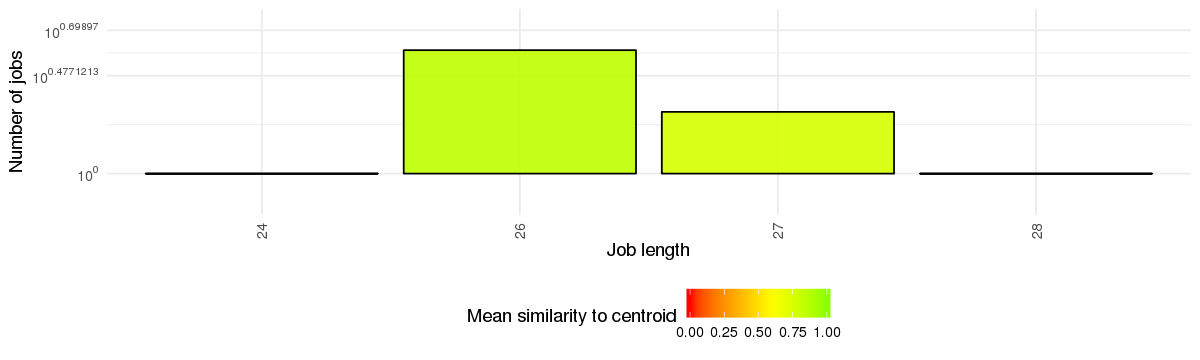
\includegraphics[width=4.61in,height=1.39in]{./media/image6.png}
	\captionof{figure}{Length distribution in the cluster.}
  \label{fig:use_case:bin_aggzeros:length}
\endgroup
%\end{figure}


\paragraph{HEX\_LEV}
Information related to the cluster is in \Cref{tab:use_case:hex_lev:stats}, \Cref{tab:use_case:hex_lev:top_jobs}, and in \Cref{fig:use_case:hex_lev:length}.

%\begin{table}[h]
\begingroup
  \centering
  \begin{tabular}{ll}
    SIM & 0.9 \\
    Number of jobs & 209 \\
    Number of job types & 189 \\
  \end{tabular}
	\captionof{table}{Cluster statistics.}
  \label{tab:use_case:hex_lev:stats}
\endgroup
%\end{table}

%\begin{table}[h]
\begingroup
  \begin{tiny}
    \begin{tabular}{@{ }l@{ }@{ }l@{ }|@{ }r@{ }}
			\rowcolor{tabhcolor}
			\multicolumn{2}{@{ }l|@{ }}{\rowstyle{\bfseries}Hexadecimal coding} & \\
			\rowcolor{tabhcolor}\rowstyle{\bfseries}
      md\_other                                           &  read\_calls                                           & Type     \\ 
      \hline
      0:\dots:0                                           &  3:3:8:8:8:5:6:8:8:8:8:8:8:8:8:8:8:8:8:8:8:8:8:8:8:8:8 & job      \\ 
      0:\dots:0                                           &  8:8:8:8:8:2:6:8:8:8:8:8:8:8:8:8:8:8:8:8:8:8:8:8:8:8:8 & centroid \\ 
      \multicolumn{3}{l}{}                                \\ 
			\rowcolor{tabhcolor}\rowstyle{\bfseries}
      md\_other                                           &  read\_calls                                           & Count    \\ 
      \hline
      0:\dots:0                                           &  0:0:0:0:0:0:8:8:8:8:8:8:8:8:8:8:8:8:8:8:8:8:8:8:8:8   & 4        \\ 
      0:\dots:0                                           &  8:8:8:8:8:2:8:8:8:8:8:8:8:8:8:8:8:8:8:8:8:8:8:8:8:8   & 4        \\ 
      0:0:0:4:0:0:0:0:0:0:0:0:0:0:0:0:0:0:0:0:0:0:0:0:0:0 &  0:0:0:0:0:0:8:8:8:8:8:8:8:8:8:8:8:8:8:8:8:8:8:8:8:8   & 4        \\ 
      0:\dots:0                                           &  8:8:8:8:8:3:8:8:8:8:8:8:8:8:8:8:8:8:8:8:8:8:8:8:8:8:8 & 3        \\ 
      0:\dots:0                                           &  0:0:0:0:0:0:2:8:8:8:8:8:8:8:8:8:8:8:8:8:8:8:8:8:8:8   & 2        \\ 
    \end{tabular}
  \end{tiny}
	\captionof{table}{Job, centroid and Top 5 job types.}
  \label{tab:use_case:hex_lev:top_jobs}
\endgroup
%\end{table}

%\begin{figure}[h]
\begingroup
  \centering
  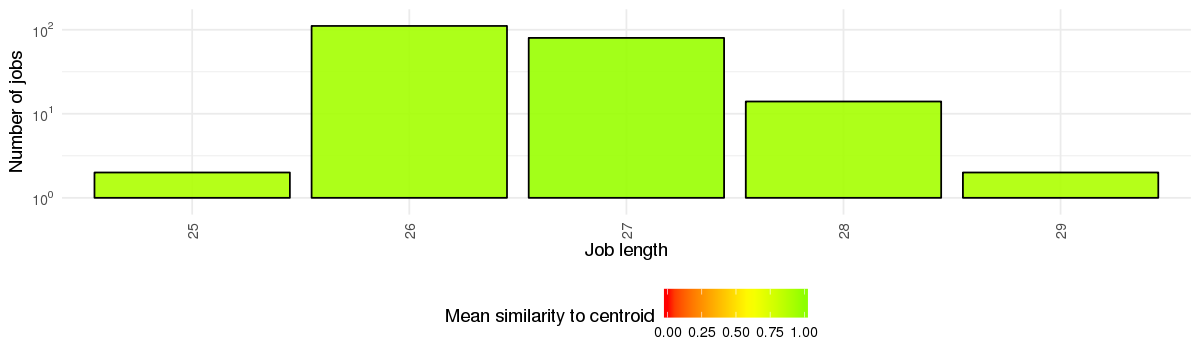
\includegraphics[width=4.61in,height=1.39in]{./media/image17.png}
	\captionof{figure}{Length distribution in the cluster.}
  \label{fig:use_case:hex_lev:length}
\endgroup
%\end{figure}


\paragraph{HEX\_NATIVE}
Information related to the cluster is in \Cref{tab:use_case:hex_native:stats}, \Cref{tab:use_case:hex_native:job_centroid}, and in \Cref{fig:use_case:hex_native:length}.

%\begin{table}[h]
\begingroup
  \centering
  \begin{tabular}{ll}
    SIM & 0.99 \\
    Number of jobs & 20 \\
    Number of job types & 20 \\
  \end{tabular}
	\captionof{table}{Cluster statistics.}
  \label{tab:use_case:hex_native:stats}
\endgroup
%\end{table}

%\begin{table}[h]
\begingroup
  \centering
  \begin{tiny}
    \begin{tabular}{@{ }l@{ }|@{ }r@{ }}
			\rowcolor{tabhcolor}\rowstyle{\bfseries}
      Hexadecimal coding & \\
			\rowcolor{tabhcolor}\rowstyle{\bfseries}
      read\_calls                                           & Type     \\ 
      \hline	
      3:3:8:8:8:5:6:8:8:8:8:8:8:8:8:8:8:8:8:8:8:8:8:8:8:8:8 & job      \\ 
      8:8:8:8:8:2:4:8:8:8:8:8:8:8:8:8:8:8:8:8:8:8:8:8:8:8:8 & centroid \\ 
      \multicolumn{2}{l}{}\\ 
			\rowcolor{tabhcolor}\rowstyle{\bfseries}
      read\_calls                                           & Count    \\ 
      \hline	
      8:8:8:8:8:3:8:8:8:8:8:8:8:8:8:8:8:8:8:8:8:8:8:8:8:8:8 & 3        \\ 
      8:8:8:8:8:5:8:8:8:8:8:8:8:8:8:8:8:8:8:8:8:8:8:8:8:8:8 & 2        \\ 
      3:3:8:8:8:5:6:8:8:8:8:8:8:8:8:8:8:8:8:8:8:8:8:8:8:8:8 & 1        \\ 
      3:6:6:7:7:7:7:8:8:8:8:8:8:8:8:8:8:8:8:8:8:8:8:8:8:8:8 & 1        \\ 
      6:5:6:7:6:2:7:8:8:8:8:8:8:8:8:8:8:8:8:8:8:8:8:8:8:8:8 & 1        \\ 
    \end{tabular}
  \end{tiny}
	\captionof{table}{Job and centroid coding sequences.}
  \label{tab:use_case:hex_native:job_centroid}
\endgroup
%\end{table}

%\begin{figure}[h]
\begingroup
  \centering
  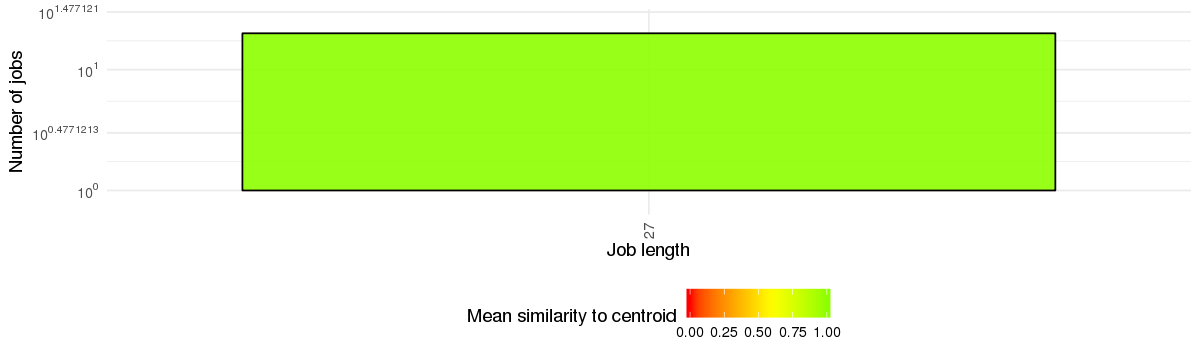
\includegraphics[width=4.61in,height=1.39in]{./media/image2.png}
	\captionof{table}{Figure 19. Length distribution in the cluster.}
  \label{fig:use_case:hex_native:length}
\endgroup
%\end{figure}


\paragraph{PM\_QUANT}
Information\ related to the cluster is \Cref{tab:use_case:pm_quant:stats}, \Cref{tab:use_case:pm_quant:top_jobs}, and in \Cref{fig:use_case:pm_quant:length}.

An attentive reader may notice that there is a discrepancy between the job visualization in \Cref{fig:use_case} and the job coding in \Cref{tab:use_case:pm_quant:top_jobs}.
While in the figure we can see a less intensive phase in the beginning and a high intensive phase afterwards, the coding contains a more or less single high intensive I/O phase.
The reason is that we use different reduction functions.
While in the illustration we aggregate segments by the sum() function, for the coding we use quantization of the performance mean value.
Mean value allow us to build simple algorithms

%\begin{table}[h]
\begingroup
  \centering
  \begin{tabular}{ll}
    SIM                 & 0.7 \\ 
    Number of jobs      & 68  \\ 
    Number of job types & 59  \\ 
  \end{tabular}
	\captionof{table}{Cluster statistics.}
  \label{tab:use_case:pm_quant:stats}
\endgroup
%\end{table}


%\begin{table}[h]
\begingroup
  \centering
  \begin{tiny}
    \begin{tabular}{@{ }l@{ }|@{ }r@{ }}
			\rowcolor{tabhcolor}\rowstyle{\bfseries}
      Hexadecimal coding & \\
			\rowcolor{tabhcolor}\rowstyle{\bfseries}
			read\_calls                                           & Type     \\ 
      \hline
      3:3:8:8:8:5:6:8:8:8:8:8:8:8:8:8:8:8:8:8:8:8:8:8:8:8:8 & job      \\ 
      8:8:8:8:8:8:8:8:8:8:8:8:8:8:8:8:8:8:8:8:8:8:8:8:8:8   & centroid \\ 
      \multicolumn{2}{l}{}\\
			\rowcolor{tabhcolor}\rowstyle{\bfseries}
      read\_calls                                           & Count    \\ 
      \hline
      8:8:8:8:8:2:8:8:8:8:8:8:8:8:8:8:8:8:8:8:8:8:8:8:8:8   & 4        \\ 
      8:8:8:8:8:3:8:8:8:8:8:8:8:8:8:8:8:8:8:8:8:8:8:8:8:8:8 & 3        \\ 
      7:7:7:7:7:2:8:8:8:8:8:8:8:8:8:8:8:8:8:8:8:8:8:8:8:8   & 2        \\ 
      8:8:8:8:8:5:8:8:8:8:8:8:8:8:8:8:8:8:8:8:8:8:8:8:8:8   & 2        \\ 
      8:8:8:8:8:8:8:8:8:8:8:8:8:8:8:8:8:8:8:8:8:8:8:8:8:8   & 2        \\ 
    \end{tabular}
  \end{tiny}
	\captionof{table}{Job, centroid and Top 5 job types.}
  \label{tab:use_case:pm_quant:top_jobs}
\endgroup
%\end{table}

%\begin{figure}[h]
\begingroup
  \centering
  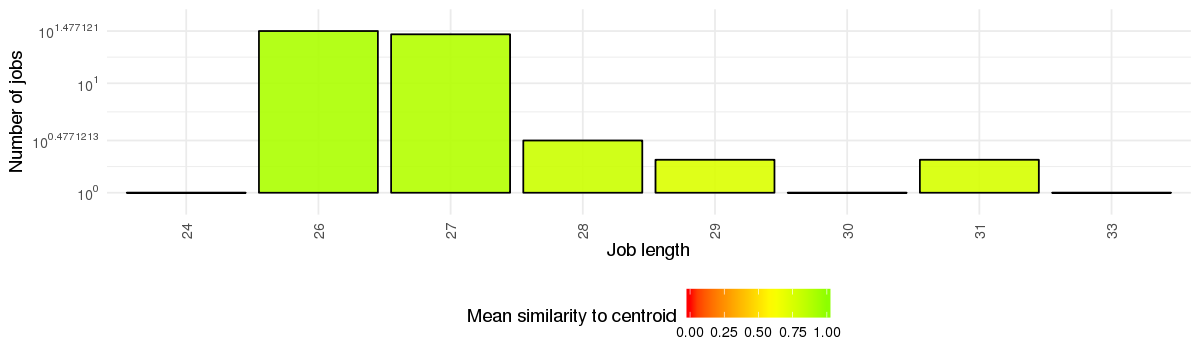
\includegraphics[width=4.61in,height=1.39in]{./media/image7.png}
	\captionof{figure}{Length distribution in the cluster.}
  \label{fig:use_case:pm_quant:length}
\endgroup
%\end{figure}

\subsubsection{Discussion}
Indeed clustering of hexadecimal codings produces usable results.
The examples in Table 2 show two randomly picked clusters.
The similar I/O behavior.

Another\ critical point of usage of Levenshtein distance is that it doesn't consider the performance.
For example, the following three codings would be considered as similar, since they differ in one position only.

\begin{lstlisting}
phase_coding_1 : [2:2:2:2:2:9:2:2]
phase_coding_2 : [2:2:2:2:2:8:2:2]
phase_coding_3 : [2:2:2:2:2:0:2:2]
\end{lstlisting}

Intuitively, we would say that {phase\_coding\_1 and{ phase\_coding\_2 are more similar than {phase\_coding\_2 and {phase\_coding\_3 , because the difference at 6th position is in the first case smaller (9 and 8) is smaller than in the second case (8 and 0).
Particularly bad affected are short coding, as the example in the previous sections shows.

The\ current version of the PM algorithm ignores non-IO parts (sequences of zeros) of the monitoring data, and  handles segment sequences like [0,0,0,0,1] and [1] equally.
These sequences would produce different average I/O loads on the storage.
Intuitively, we would say these jobs have different I/O behaviour and should consider that in the approach.

\begin{lstlisting}
job1_metric1 : [0,0,0,0,1]
job1_metric1 : [1]
\end{lstlisting}

One could also argue that the phase definition was chosen incorrectly.
Currently, phases are defined for each metric individually, without consideration what is going on on other metrics.
For illustration, consider the following two jobs.
Currently, the algorithm recognizes the I/O pattern as 100$\%$  similar.
Alternatively, one could say that running two metrics at the same time is another I/O pattern, as running them shifted, because on a storage system the jobs would produce different I/O loads.

\begin{lstlisting}
job1_metric1 : [0:1]
job1_metric2 : [1:0]
job2_metric1 : [1:0]
job2_metric2 : [1:0]
\end{lstlisting}

The benefit of ignoring these both aspects is simplicity.
This reduces the number of clusters and the results are easier to understand.
It also needs to be investigated, if these considerations are correct for HPC systems that are running hundreds of jobs in parallel, because one job alone would typically not be able to produce a significant amount of I/O that can slow down the file system performance.

The success of general purpose clustering and classification algorithms depends on right feature selection and data transformation.
In particular, feature selection is often quite challenging.
This makes training of models a kind of try and error approach.
Even if an optimal solution is found there is no guarantee that the approach with other data on other systems.

As you might have noticed, quantization is not necessary for PM.
It can perfectly work directly with floating point numbers, such as mean performance values.
The main motivation behind the use of hexadecimal coding is that it makes PM comparable with other algorithms.
For example, this allows us to see how the additional features affect the quality of clusters.
By accident, this was also the right decision.
We noticed that in the experiments with floating point numbers the amount of generated clusters skyrocketed.
The reason is that similarity for short jobs exceeds SIM value very fast and this leads to the creation of new clusters, which in turn leads to long clustering runtimes.
An example illustrates a typical case.
Assume there are two jobs: one running on 16 nodes and other running on 32 nodes.
Both are one segment long and only one I/O node that writes data to storage with a moderate performance.
Without quantization we would represent these jobs by the following sequences:  [..., [0.0625], $ \ldots $ ] and [..., [0.03125], ...], where only active metrics have values larger than zero.
Using the similarity function without quantization, i.e.
with mean performance, would result in a similarity of 50$\%$ , and for SIM>0.5 they would be placed in separate clusters.

The hexadecimal coding filters these jobs automatically. Segments with mean performance less than 0.125 are quantized to zero and zero sequences are removed from the dataset. This problem doesn't occur.
Nevertheless, we think that we will overcome this problem in the future.
S would make the results more precise and would make the quantization step
obsolete.

\subsection{Conclusion}
After a series of experiments with general purpose algorithms we could not achieve optimal results.
The investigation of resulting clusters shows that they are obviously polluted.
One problem might be that we apply a combination of a clustering and a classification algorithm.
The classification algorithm is trained by the potential erroneous output of the clustering algorithm and it can itself produce erroneous output, which multiples the total error.
Another problem might be that both algorithms are not aware of I/O performance and I/O phases.
As this work shows, this might be quite important.
At least, we achieve better results by considering both aspects.


The Levenshtein-distance based algorithms produce better, but still not sophisticated results.
This is a direct consequence of the usage of the Levenshtein distance, which is illustrated in the following example.
Suppose two jobs {[0:6:0:0]and [0:388:174:0] are in the same cluster with the centroid {[0:388:0:0].
Even if in both cases the similarity between the cluster and the centroid is 75$\%$  (only one change is required), we would intuitively say that these jobs are completely different, not even close to the 75$\%$  mark.
We can easily construct another sequence, e.g., {[0:389:0:0], where the 75$\%$  are justified.
The reason for such clustering failures, ist that Levenshtein distance is not able to extract and to use the meaning that was coded into the numbers.

Job comparison by means of hexadecimal coding is more precise, because hexadecimal coding sequences are much longer.
Absolute coding aggregates three dimensions (Metric, Nodes, and FileSystems) resulting in a nine times shorter coding sequence than hexadecimal coding, which aggregates only two dimensions (Nodes, and FileSystems).
Having more data, a more precise computation.
The integration of the awareness of I/O performance produces better, but still not sophisticated results.
We suppose that the I/O phase awareness is the missing feature for success.

The final algorithm that detects phases and differentiates performance values produces at first sight clean results.
Due to the huge amount of clusters and lack of automatic evaluation tools, we can not prove this statement for all clustres.

\subsection{Future work}
We see a high potential in the new clustering algorithm, but it requires some improvements to be useful.
Although groping seems to work well, the algorithm has at least one serious issue.
The biggest problem is probably the large number of clusters.
We assume that there indeed are so many different types of jobs, but there are too many of them for manual labeling.
Therefore we need at least three further functions, that filter irrelevant clusters, sort clusters by a criteria and label remaining ones.


%\setlength{\parskip}{0.0pt}
%\begin{thebibliography}{99}
%\bibitem{item1}
%\fontsize{10pt}{12.0pt}\selectfont Ahn, D., Garlick, J., Grondona, M., Lipari, D., Springmeyer, B., Schulz, M.: Flux: $``$A next-generation resource management framework for large hpc centers.$"$  pp. 9-17 (09 2014). \href{https://doi.org/10.1109/ICPPW.2014.15}{\textcolor[HTML]{1155CC}{\ul{https://doi.org/10.1109/ICPPW.2014.15}}}

%\bibitem{item2}
%\fontsize{10pt}{12.0pt}\selectfont DDN, $``$Worlds's most advanced application aware I/O acceleration solutions.$"$  \href{http://www.ddn.com/products/infinite-memory-engine-ime14k}{\textcolor[HTML]{1155CC}{\ul{ http://www.ddn.com/products/infinite-memory-engine-ime14k}}}

%\bibitem{item3}
%\fontsize{10pt}{12.0pt}\selectfont IBM, $``$Flash Storage.$"$ ,\href{http://www-03.ibm.com/systems/storage/flash}{\textcolor[HTML]{1155CC}{\ul{ http://www-03.ibm.com/systems/storage/flash}}}

%\bibitem{item4}
%\fontsize{10pt}{12.0pt}\selectfont Kove Corporation, $``$about xpress disk (xpd)$"$ , 2015

%\bibitem{item5}
%\fontsize{10pt}{12.0pt}\selectfont Kunkel,\ J., Zimmer, M., Hübbe, N., Aguilera, A., Mickler, H., Wang, X., Chut, A., Bönisch, T., Lüttgau, J., Michel, R., Weging, J., $``$The SIOX Architecture - Coupling Automatic Monitoring and Optimization of Parallel I/O.$"$ ,  In: Kunkel, J., Ludwig, T., Meuer, H. (eds.) Supercomputing. pp. 245-260. Supercomputing, ISC events, Lecture Notes in Computer Science, 2014

%\bibitem{item6}
%\fontsize{10pt}{12.0pt}\selectfont Liang, W., Chen, Y., Liu, J., An, H.: Cars, $``$A contention-aware scheduler for efficient resource management of hpc storage systems.$"$ , Parallel Computing 87, 25 - 34, 2019 \href{https://doi.org/https://doi.org/10.1016/j.parco.2019.04.010}{\textcolor[HTML]{1155CC}{\ul{https://doi.org/https://doi.org/10.1016/j.parco.2019.04.010}}}, \href{http://www.sciencedirect.com/science/article/pii/S016781911830382X}{\textcolor[HTML]{1155CC}{\ul{http://www.sciencedirect.com/science/article/pii/S016781911830382X}}}

%\bibitem{item7}
%\fontsize{10pt}{12.0pt}\selectfont Sivalingam, K., Richardson, H., Tate, A., Lafferty, M.: Lassi, $``$Metric based i/o analytics for hpc$"$ , 2019

%\bibitem{item8}
%\fontsize{10pt}{12.0pt}\selectfont Snyder, S., Carns, P., Harms, K., Ross, R., Lockwood, G.K., Wright, N.J., \\
%$``$Modular hpc i/o characterization with darshan.$"$  In: 2016 5th Workshop on Extreme-Scale Programming Tools (ESPT). pp. 9-17, 2016

%\bibitem{item9}
%\fontsize{10pt}{12.0pt}\selectfont Kunkel, J., Markomanolis, G.,:Understanding Metadata Latency with MDWorkbench, In High Performance Computing: ISC High Performance 2018 International Workshops, Frankfurt/Main, Germany, June 28, 2018, Revised Selected Papers, Lecture Notes in Computer Science (11203), pp. 75-88, Springer, WOPSSS workshop, ISC HPC, Frankfurt, Germany, ISBN: 978-3-030-02465-9, \href{https://doi.org/10.1007/978-3-030-02465-9_5}{\textcolor[HTML]{1155CC}{\ul{https://doi.org/10.1007/978-3-030-02465-9\_5}}}

%\bibitem{item10}
%\href{http://jmlr.csail.mit.edu/papers/v12/pedregosa11a.html}{{\fontsize{10pt}{12.0pt}\selectfont \textcolor[HTML]{1155CC}{\ul{Scikit-learn: Machine Learning in Python}}}, Pedregosa \textit{et al.}, JMLR 12, pp. 2825-2830, 2011.

%\bibitem{item11}
%\fontsize{10pt}{12.0pt}\selectfont Betke, E., Kunkel. J.: Semi-automatic Assessment of I/O Behavior by Inspecting the Individual Client-Node Timelines -- An Explorative Study on 10$ \string^ $ 6 Jobs, ISC 2020 (Submission accepted, not published yet).
%\end{thebibliography}

%\printbibliography
%\newpage
%\clearpage
%\pagebreak
\null
\bibliographystyle{splncs04}
\bibliography{bibliography}{}
\end{document}

